\chapter{TLS - Transport Layer Security}
I principali \textit{network security protocol} sono \textbf{SSH}, \textbf{SSL} (\textit{secure socket layer}), \textbf{TSL} e \textbf{IPsec}. Storicamente il primo pensato fu SSL, realizzato in diverse versioni ognuna sempre migliore, fino a quella che conosciamo oggi. Facciamo un breve recap storico:
\begin{itemize}
    \item (\textbf{1994}) SSL v1 viene sviluppato da \textit{Netscape} ma mai rilasciato.
    \item (\textbf{1995}) SSL v2 viene integrato in \textit{Netscape 1.1} e verrà successivamente rotto.
    \item(\textbf{1996}) SSL v3 vene ridisegnato dalla base da \textit{Netscape}.
    \item(\textbf{1996-1999}) TLS v1.0 viene sviluppato parallelamente a \textit{SSL} dalla \textbf{IETF}, partendo dalla sua versione 3.1. Il protocollo è basato interamente su \textit{TCP} per la parte di trasmissione e integra algoritmi di sicurezza \textbf{\textit{hardcoded}}.
    \item(\textbf{2006}) TLS v1.1 viene rilasciato e viene aggiunto il supporto a \textit{UDP}. 
    \item(\textbf{2008}) TLS v1.2 viene rilasciato per disaccoppiare i sistemi di sicurezza deboli come \textit{MD5/SHA-1} precedentemente hardcoded nel sistema. Introduce il concetto di \textit{Negotiated-PRF}, impostando come default \textit{SHA-256}.
    \item(\textbf{2018}) \textbf{TLS v1.3 viene rilasciato, costituendo un nuovo protocollo}. Vengono introdotti e ammessi solo cifratori basati su \textit{AEAD} e viene aggiunto il \textbf{\textit{Threeway-Handshake}}
\end{itemize}
\begin{remark}
TLS v1.3 rimuove anche \textbf{RSA}, in quanto il modo in cui viene usato può portare a diversi problemi.
\end{remark}
In ultimo è utile ricordare che:
\begin{proposition}[Livelli di Protezione]
SSL/TLS sono protocolli di protezione che vanno \textbf{sopra} lo strato di trasmissione e sotto quello applicativo. Tuttavia non vanno presi come un miglioramento alla sicurezza di TCP in quanto i servizi offerti da TLS non sono limitati al garantire un trasporto sicuro di dati e descrivono una più generale relazione point-to-point.\\
Questo significa che SSL/TLS proteggono \textbf{esclusivamente}\footnotemark il payload di un determinato pacchetto.
\footnotetext{\textsuperscript{\thefootnote}IPsec protegge invece tutto il pacchetto, sia payload che header.}
\end{proposition}
\section{Il Supporto Applicativo}
Quando un servizio applicativo viene standardizzato bisogna specificare una serie di parametri come \textbf{IP address} e \textbf{port number} del servizio. TLS, avendo una \textit{struttura a strati}, riesce a fornire un supporto ben strutturato a questa modalità di sviluppo poiché l'applicazione utilizza nel suo pacchetto la porta del servizio applicativo da usare (es: HTTP) mentre lo strato TLS incapsula il valore di porta specificando il valore del servizio su cui c'è sicurezza.
\begin{example}
Supponiamo di inviare un pacchetto email tramite protocollo HTTP, che usa la porta 80. Poiché il servizio di mail offerto dal protocollo SMTP usa la porta 25, l'applicazione che utilizziamo per spedire il pacchetto specificherà nell'header la porta 80 e la porta 25. Se la connessione che usiamo è protetta da TLS, prima che il pacchetto venga passato allo strato di trasporto verranno specificate nuove porte, rispettivamente 443 per HTTPS e 587 per SMTPS, le due versioni sicure dei protocolli precedenti. 
\end{example}
\begin{figure}[H]
    \centering
    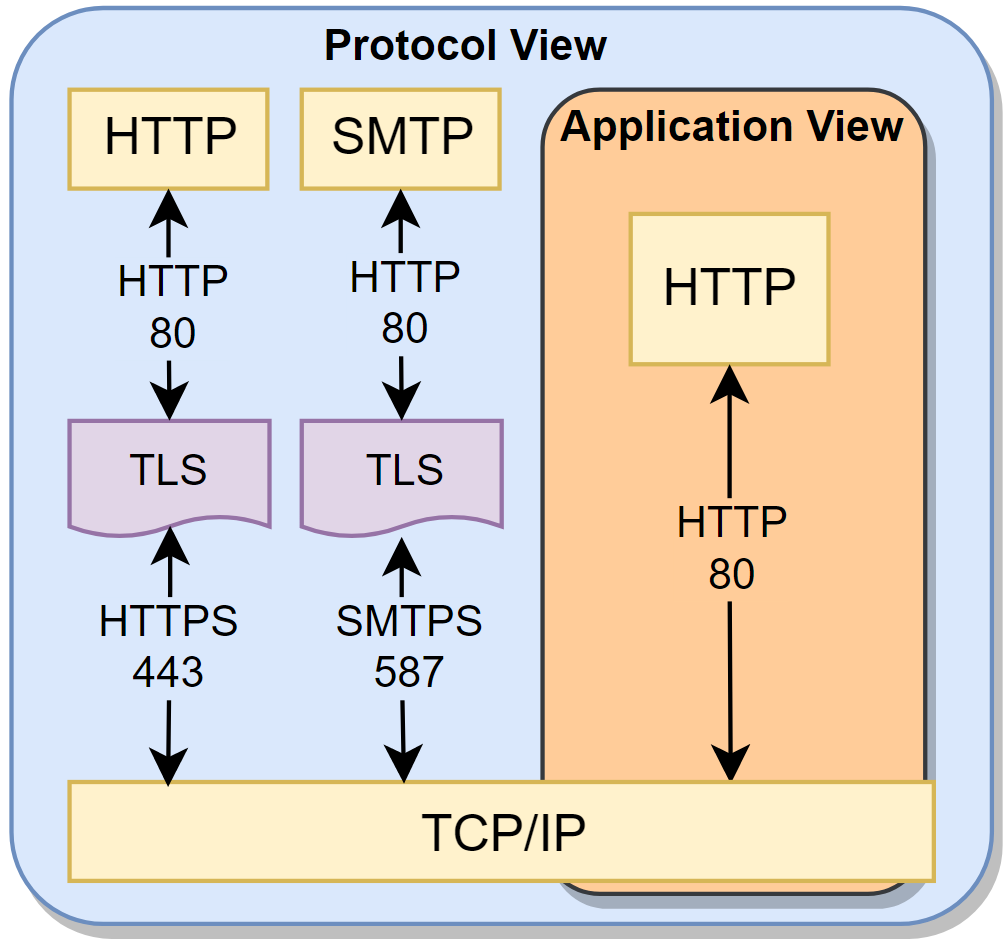
\includegraphics[width=0.5\textwidth]{image/tlsencapsulation.png}
    \caption{Port change made by TLS layer}
    \label{fig:tlsencapsulation}
\end{figure}
\begin{remark}
Le ragioni dietro questa scelta sono prettamente storiche. All'inizio nessuno usava TLS al di fuori delle comunicazioni di rete e si voleva garantire la scelta di utilizzare un servizio piuttosto che un altro, comportando una duplicazione delle porte per una medesima applicazione.
\end{remark}
\begin{remark}
IPsec usa un servizio chiamato \textbf{traffic flow confidentiality} che impedisce ad una persona intenta ad osservare il flusso dati in trasmissione quale protocollo/applicazione stiamo utilizzando. In TLS questo servizio \textbf{NON C'E'}, quindi l'applicazione e il protocollo appaiono in chiaro.
\end{remark}
\begin{remark}
Analizziamo da ora in poi TLS v1.2, evidenziando alcune differenze con la v1.3.
\end{remark}
\section{TLS Protocol Stack}
Abbiamo detto che TLS nasce per garantire una connessione sicura. Vediamo quali sono i servizi che dobbiamo garantire per averla e il modo con cui vengono forniti. TLS deve:
\begin{proposition}[TLS Services]
\begin{enumerate}
    \item Creare una sessione (Handshake Phase)
    \item Condividere dei segreti.
    \item permettere autenticazione degli utenti.
    \item Trasferire dati su un canale sicuro (Symmetric Encryption).
    \item Garantire integrità dei dati trasmessi (HMAC).
\end{enumerate}
\end{proposition}
Il modo con cui TLS fornisce questi servizi è quello di fare due operazioni insieme, per motivi storici, a differenza di altri protocolli come IPsec che distinguono bene la fase di creazione della sessione da quella di trasferimento.\\
\begin{wrapfigure}{r}{0.5\textwidth}
\vspace{-7mm}
    \centering
    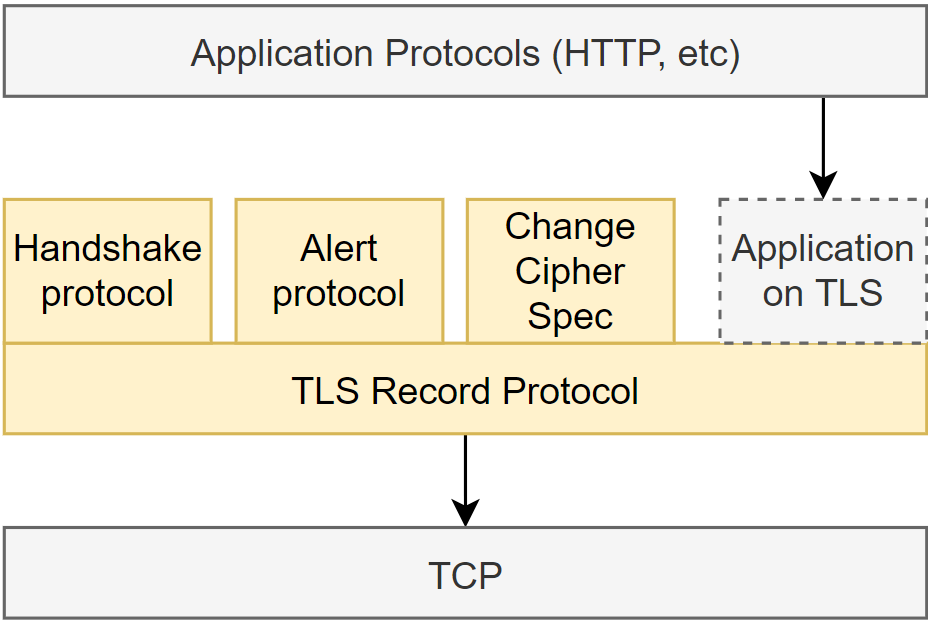
\includegraphics[width=0.5\textwidth]{image/tlsstack.png}
    \caption{TLS Protocol Stack}
    \label{fig:tlsstack}
\end{wrapfigure}
Lo stack di protocollo è quello visibile in \cref{fig:tlsstack}. Abbiamo detto che TLS fa un incapsulamento del pacchetto per rimappare la porta e specificare che si sta usando un servizio protetto; questo avviene nel \textit{TLS Record Protocol}, al di sopra del quale possono essere eseguite applicazioni, l'handshake protocol e si possono gestire anche alert secondo protocolli variabili. \\Il blocco relativo alle specifiche di cifratura serve per segnalare che il servizio di cifratura è attivo.
\subsection{TLS Record Protocol}
Il \textbf{\textit{Record Protocol}} si occupa di prendere il messaggio trasmesso dall'applicazione per trasformarlo in uno coerente con le specifiche del protocollo. Le operazioni sono le seguenti:


\noindent\begin{minipage}{0.6\textwidth}
\vspace{4pt}
\begin{theorem}[Record Protocol - Send]\label{thm:recordprotocolsnd}
\begin{itemize}
    \item \textbf{Recupero Dati:} prelievo del messaggio generato dall'applicazione.
    \item \textbf{Frammentazione:} Divide i messaggi in frammenti di dimensioni gestibili.
    \item \textbf{Compressione (opzionale)}
    \item \textbf{Generazione MAC:} genera il MAC e appendilo in coda.
    \item \textbf{Criptazione:} Cifra il pacchetto e il MAC.
    \item \textbf{Aggiungi Header TCP:} aggiungere l'header con le informazioni protocollari in testa.
\end{itemize}
\end{theorem}
\end{minipage}
\hspace{0.05\textwidth}
\begin{minipage}{0.4\textwidth}\vspace{4pt}
%\begin{figure}[h]
\centering
\captionsetup{type=figure}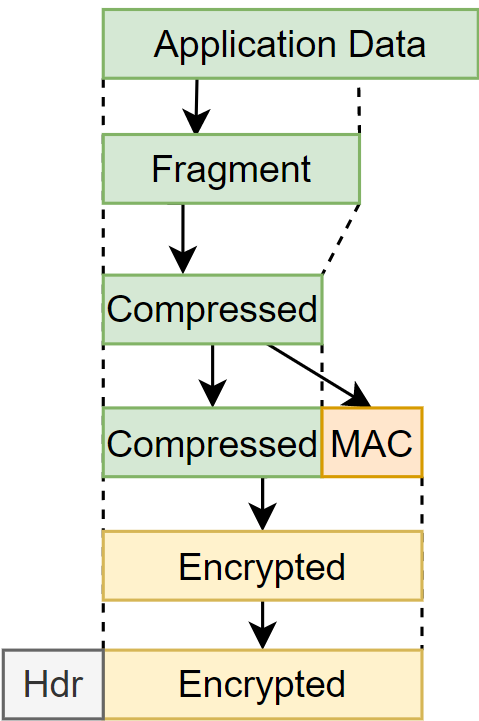
\includegraphics[width=0.7\textwidth]{image/tlsrecord.png}
%\caption{TLS Record Protocol}
\captionof{figure}{TLS Record Protocol}
\label{fig:tlsrecord}
%\end{figure}
\end{minipage}
\begin{theorem}[Record Protocol - Receive]\label{thm:recordprotocolrcv}
\begin{enumerate}
    \item Decifra il Pacchetto.
    \item Calcola il MAC e verifica con quello trasmesso.
    \item \textbf{(opzionale)} Decomprimi.
    \item Riassembla i frammenti.
    \item Trasmetti al livello applicativo il messaggio.
\end{enumerate}
\end{theorem}
Nel Record Protocol è possibile notare il primo grande errore delle versioni antecedenti\footnote{Nella v1.0/SSL v3 venne considerata l'ipotesi della compressione, ma non venne applicata.} alla 1.3. Il meccanismo di \textbf{compress-than-MAC and encrypt} infatti rendeva possibile un particolare attacco (molto complesso) di cui parleremo più avanti. Analizziamo ora i punti del protocollo:

\begin{itemize}
    \item La compressione è di tipo \textit{loseless}\footnote{Senza perdita di informazioni.} e viene fatta prima di cifrare, in quanto non avrebbe senso cercare una logica di compressione nel digest (serve un messaggio a bassa entropia).\footnote{Una compressione può essere tipo $f(AAAA) = 4A$. In un messaggio (pseudo)randomico non avrebbe senso.}
    \item Il MAC viene generato con una \textbf{HMAC-construction} (\cref{def:hmac}) tramite chiave simmetrica scambiata durante il set-up dei parametri di sicurezza negoziati in fase di hanshake, così come l'hash-function.
    \item La cifratura è applicata al singolo fragment e al suo MAC (possibilmente compressi) e non sarebbe possibile senza una negoziazione iniziale. L'algoritmo usato è un block o stream cipher (\cref{chap:blkcipher}, \cref{chap:streamcipher}), anch'esso deciso in fase di negoziazione ma la dimensione del digest non deve superare 1024 bytes.
\end{itemize}
La parte relativa ai dati trasmessi del Record Protocol (\cref{fig:tlsstack}) è una struttura dati con i seguenti campi:
\begin{definition}[Record Protocol Data Unit]
\begin{itemize}
    \item \textbf{Header (5 bytes)}, costituito da:
    \begin{itemize}
        \item \textbf{Content Type (1 byte):} specifica il protocollo a livello superiore da attuare. Valori che può assumere sono: \textbf{20} per \textbf{Change Cipher spec}, \textbf{21} per un messaggio di \textbf{Alert}, \textbf{22} per la \textbf{fase di handshake}, \textbf{23} se sono dati applicativi.
        \item \textbf{Versione (1 byte):} vengono specificate la minima e massima versione supportata dal sistema. 
        \item \textbf{Lunghezza (2 byte)}.
    \end{itemize}
    \item \textbf{Ciphertext}, occasionalmente compresso.
    \item \textbf{MAC}.
\end{itemize}
\begin{remark}
Poiché TLS si appoggia, generalmente, a TCP non è necessario includere un SQN in quanto il protocollo di trasporto garantisce che i pacchetti arrivino in ordine.
\end{remark}
\end{definition}
\begin{remark}[\textbf{Replay Attack}]
Come detto nella \cref{prop:macreplay} un \textbf{MAC non protegge da replay attack} a meno che questo non venga calcolato on-the-fly includendo una nonce. Nel caso di TLS \textbf{venne usato} un \textbf{SQN}, \textbf{inizializzato a 0} e con \textbf{massimo $2^{64}-1$}, mantenuto in modo separato agli estremi della connessione.\\
Poiché come detto TLS si appoggia a TCP, \textbf{per ottimizzare} il protocollo \textbf{non venne specificato} un sequence-number ma venne \textbf{usato} direttamente \textbf{quello} di \textbf{TCP} \textbf{per} eseguire \textbf{il calcolo del MAC} \textbf{senza} mai \textbf{includerlo nel pacchetto} trasmesso. 
\end{remark}
\begin{remark}[\textbf{Cambiamento in DTLS}]
\textbf{\textcolor{red}{Per includere UDP come protocollo di trasmissione è stato necessario specificare un sequence di 8 bytes.}}
\end{remark}
\begin{remark}
Includere un sequence number come nonce permette di individuare dati extra o mancanti e di prevenire replay/reordering attack.
\end{remark}

\section{Handshake Protocol}
TLS si fonda sul protocollo di Handshake che permette di fare una \textit{negoziazione} iniziale e di scambiare tutti i parametri necessari alla creazione di una \textbf{sessione sicura}, oppure per riavviare una sessione precedentemente aperta.
\begin{proposition}[Session Init Steps (overview)]
\noindent
\begin{enumerate}
    \item Effettuare la \textbf{mutua autenticazione}(\cref{chap:mutualauth}) di client e server.
    \item \textbf{Accordarsi} sugli \textbf{algoritmi} da utilizzare.
    \item \textbf{Scambio} di \textbf{valori casuali}
    \item \textbf{Scambio} di \textbf{segreti} e/o \textbf{informazioni} necessarie a \textbf{derivare} le \textbf{chiavi}
\end{enumerate}
\end{proposition}
\begin{proposition}[Session Restart (overview)]
Viene effettuato un \textbf{handshake abbreviato} per fare \textbf{rekeying}; devono essere \textbf{generati nuovi segreti} da cui \textbf{derivare nuove chiavi} di sessione.
\end{proposition}
L'obiettivo della procedura di handshake è quindi quella di fornire un protocollo unico che raccoglie i seguenti servizi:
\begin{theorem}[Handshake Protocol's Duties]
\noindent
\begin{itemize}
    \item \textbf{Negoziazione Sicura di Segreti Condivisi:} per garantire la \textbf{confidenzialità} dei \textbf{segreti condivisi} viene usata crittografia asimmetrica.
    \item \textbf{Negoziazione Affidabile:} un'attaccante \textbf{NON} deve essere in grado di \textbf{modificare/alterare} una \textbf{negoziazione} senza che venga rilevato dal protocollo.
    \item \textbf{Autenticazione Opzionale:} deve essere possibile \textbf{scegliere} quali delle parti autenticare.
    \item \textbf{Autenticazione Sicura:} il meccanismo di auth deve essere \textbf{robusto} a \textbf{MITM}.
    \end{itemize}
\end{theorem}
Il protocollo è \textbf{suddiviso in 4 fasi} ed è detto \textit{\textbf{4-way handshake}}. Ogni messaggio ha il formato seguente:
\begin{definition}[Handshake Message Format]\label{def:handshakeform}
\begin{itemize}
    \item \textbf{Header:} (4 byte) informazioni riguardanti il messaggio di handshake. Ha due campi:
    \begin{itemize}
        \item \textbf{Handshake Type:} (1 byte) indica il tipo di messaggio.
        \item \textbf{Length:} (3 byte) indica la lunghezza in byte del payload.
    \end{itemize}
    \item \textbf{Payload:} contiene le informazioni del messaggio.
\end{itemize}
I messaggi di Handshake sono \textbf{incapsulati} come \textbf{payload} all'interno del \textbf{TLS Record} (\cref{fig:tlsrecord})
\end{definition}
Il protocollo, nella sua interezza, è illustrato in \cref{fig:handshakeprot}. Nelle sezioni successive vediamo passo passo le 4 fasi.
\begin{figure}[H]
    \centering
    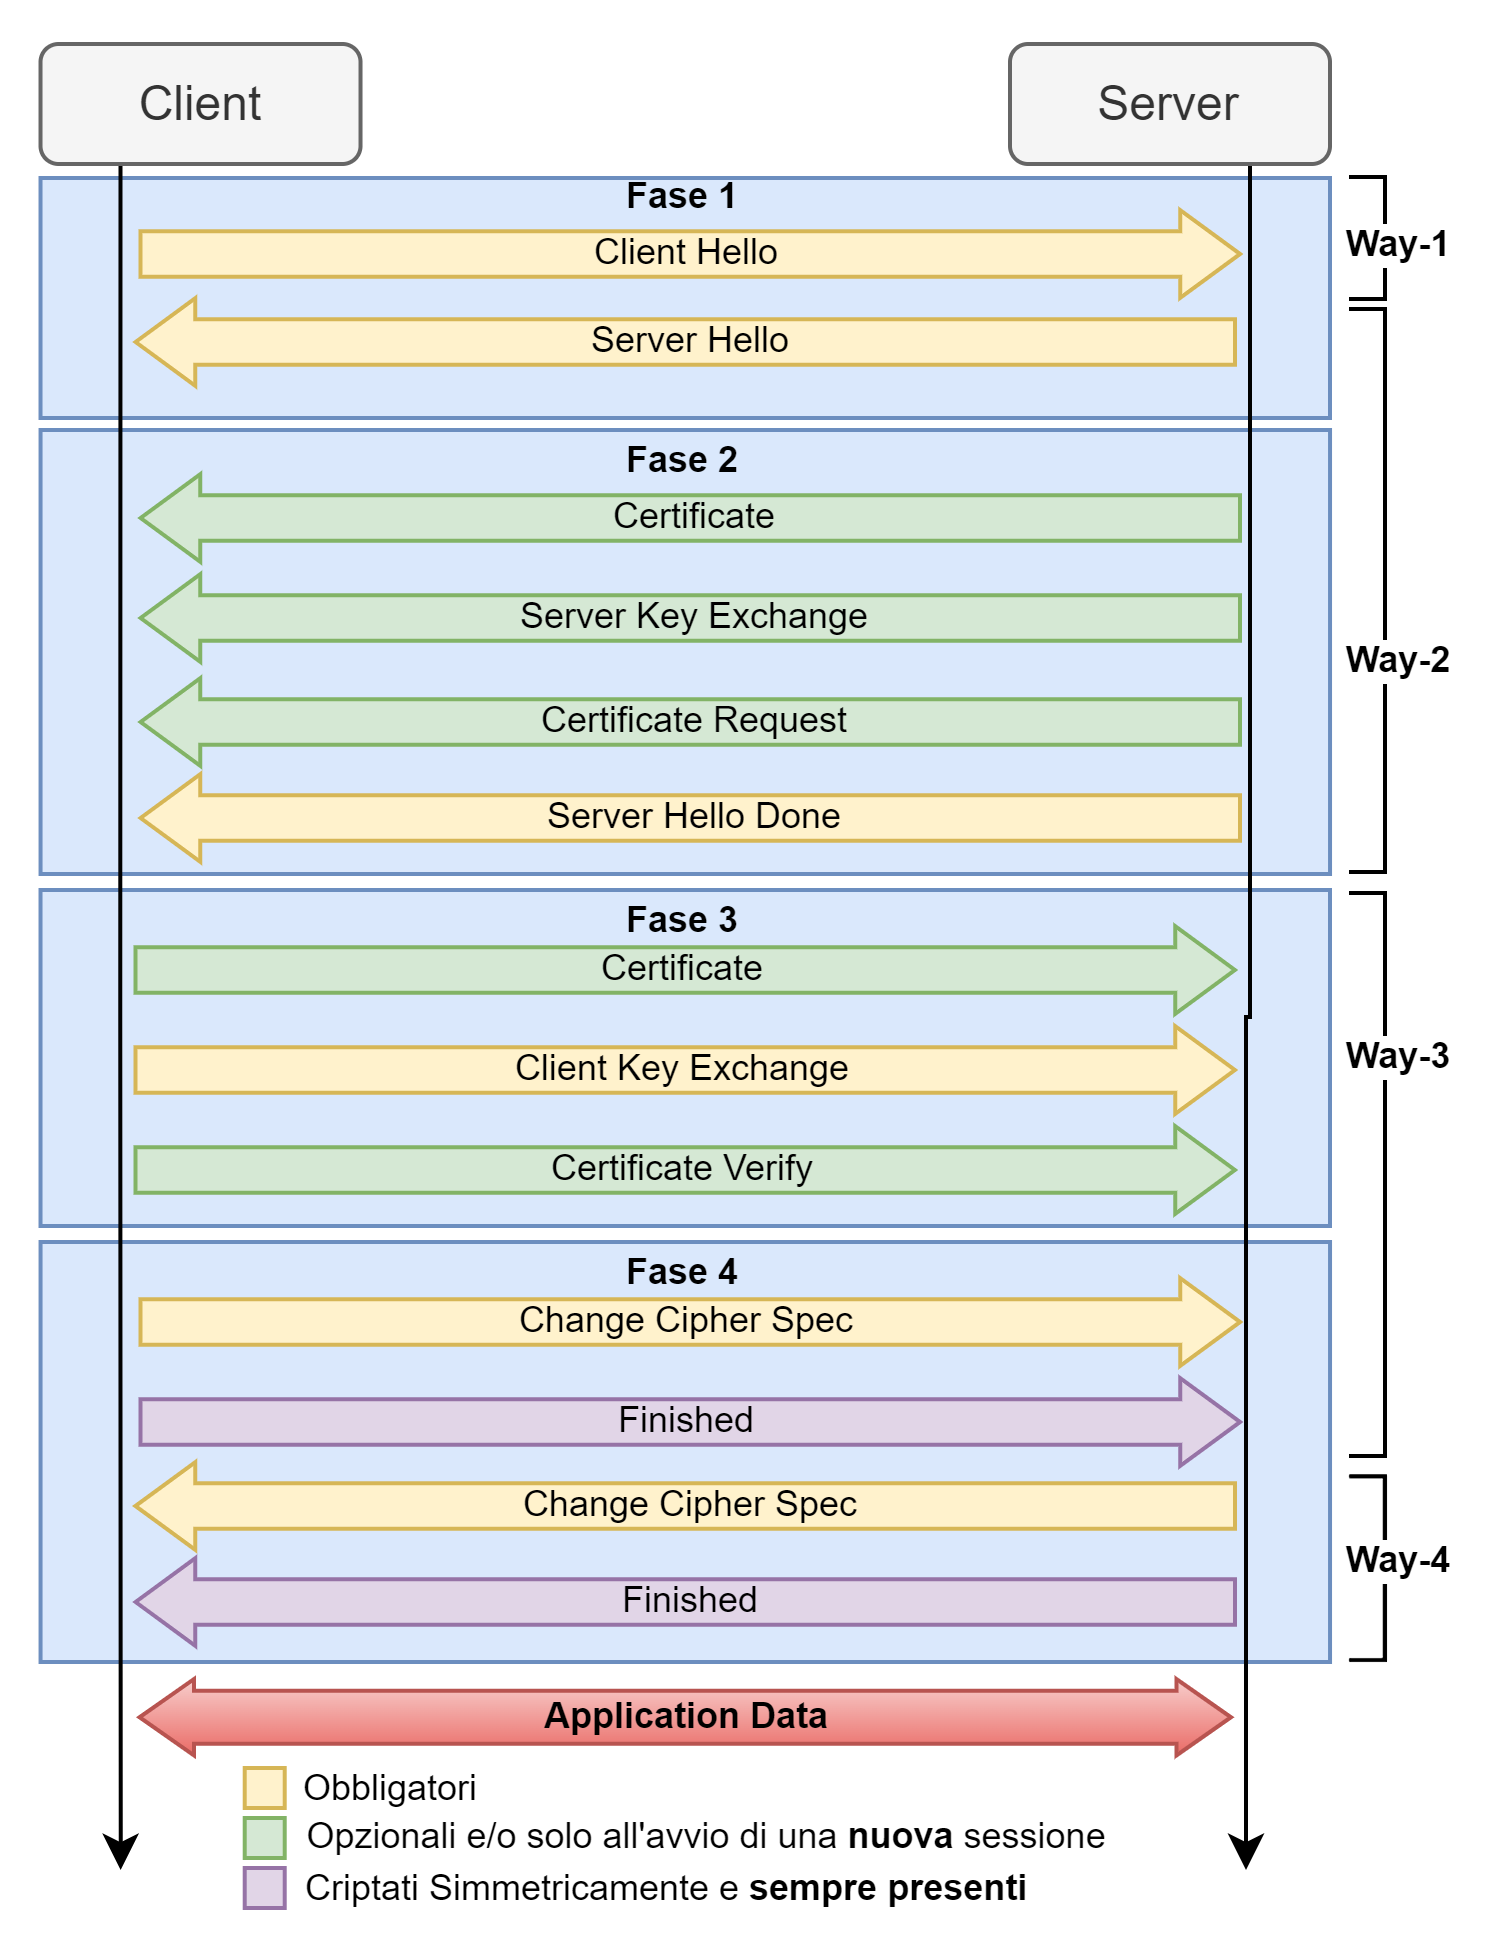
\includegraphics{image/tlshandshake.png}
    \caption{TLS Handshake Protocol}
    \label{fig:handshakeprot}
\end{figure}
\subsection{Fase 1: Hello}
La fase 1 dell’handshake ha lo scopo di creare una connessione TLS tra client e server. In particolare, svolge i seguenti compiti:
\begin{proposition}[Phase 1]
La fase uno deve:
\begin{itemize}
    \item Accordare le parti sulla \textbf{versione di TLS} da utilizzare.
    \item Definire l'\textbf{ID} della sessione.
    \item Far scambiare a entrambe le parti una \textbf{nonce} costituita da un \textbf{timestamp} e da un \textbf{valore casuale}.
    \item Accorda le parti sugli \textbf{algoritmi} di \textbf{criptazione} da utilizzare.
    \item Accorda le parti sull'\textbf{algoritmo} di \textbf{compressione} da utilizzare.
\end{itemize}
\end{proposition} 
Vengono scambiati i seguenti messaggi
\begin{definition}[Phase 1 Messages]\label{def:phase1}
\begin{enumerate}
    \item \textbf{Client Hello:} Viene inviato dal \textbf{client} \textbf{in chiaro}.
    \item \textbf{Server Hello:} Viene inviato dal \textbf{server in chiaro}.
\end{enumerate}
\end{definition}
Vediamoli nel dettaglio:
\begin{definition}[Client Hello Message]\label{def:clienthello}
\begin{itemize}
    \item \textbf{Handshake Type:} (1 byte) Indica che il messaggio è un client hello.
    \item \textbf{Length:} (3 byte) lunghezza in byte del messaggio.
    \item \textbf{Version:} (2 byte) indica la versione del protocollo TLS.
    \item \textbf{Nonce:} (32 byte) freschezza del messaggio. E' composta da:
    \begin{itemize}
        \item \textbf{Timestamp:} (4 byte) preso all'istante di generazione del messaggio.
        \item \textbf{Random Value:} (28 byte): valore casuale.
    \end{itemize}
    \item \textbf{Session ID Length:} (1 byte) lunghezza in byte dell'ID di sessione.
    \item \textbf{Session ID:} (32 byte) identifica la sessione TLS. Se corrisponde all'ID di una \textbf{precedente} sessione allora il client sta \textbf{riavviando} una \textbf{vecchia sessione.}
    \item \textbf{Cipher Suites Length:} (2 byte) indica il numero di cipher suites disponibili.
    \item \textbf{Cipher Suites:} (2 byte $\times$N) lista dei cipher algo disponibili.
    \item \textbf{Compression Length:} (1 byte) indica il numero di algoritmi di compressione disponibili.
    \item \textbf{Compression Algorithms:} (1 byte $\times$N) lista degli algoritmi di compressione disponibili.
\end{itemize}
\end{definition}
\begin{definition}[Server Hello Message]\label{def:serverhello}
\begin{itemize}
       \item \textbf{Handshake Type:} (1 byte) Indica che il messaggio è un client hello.
    \item \textbf{Length:} (3 byte) lunghezza in byte del messaggio.
    \item \textbf{Version:} (2 byte) indica la versione del protocollo TLS.
    \item \textbf{Nonce:} (32 byte) freschezza del messaggio. E' composta da:
    \begin{itemize}
        \item \textbf{Timestamp:} (4 byte) preso all'istante di generazione del messaggio.
        \item \textbf{Random Value:} (28 byte): valore casuale.
    \end{itemize}
    \item \textbf{Session ID Length:} (1 byte) lunghezza in byte dell'ID di sessione.
    \item \textbf{Session ID:} (32 byte) identifica la sessione TLS. Se l'\textbf{ID del client hello} è 0, o è di una sessione per il server \textbf{non riavviabile}, genera un nuovo ID. Altrimenti usa quello fornito dal client.
    \item \textbf{Cipher Suites:} (2 byte $\times$N) lista dei cipher algo selezionati dal Client.
    \item \textbf{Compression Algorithms:} (1 byte $\times$N) lista degli algoritmi di compressione selezionti dal client.
\end{itemize}
\end{definition}
\begin{corollary}[Cipher Suite]
Una suite di cifratura, denominata anche suite di crittografia o con il termine in inglese cipher suite è un insieme di algoritmi utilizzati per rendere sicuri i collegamenti di rete basati su TLS/SSL. L'insieme di algoritmi che costituisce una suite comprende tipicamente: un algoritmo per lo scambio delle chiavi crittografiche, un algoritmo di crittografia ed un algoritmo di message authentication code (MAC).\\
Il formato con cui una suite è definita è il seguente:
\[\text{TLS\_ASYMALGO\_WITH\_SYMALGO\_HASHALGO}\]
\begin{remark}
Non tutte le combinazioni di ASYMALGO, SYMALGO e HASHALGO sono possibili e/o proposte dal client.
\end{remark}
\end{corollary}
\subsection{Fase 2: Server Authentication}
La fase 2 due scopi:
\begin{proposition}[Phase 2]\label{prop:phase2}
\begin{itemize}
    \item \textbf{Autenticazione} (opzionale) del server, utilizzando il suo certificato.
    \item \textbf{Inviare} la \textbf{chiave pubblica} del \textbf{server} al client tramite \textbf{certificato} o messaggio extra apposito.
\end{itemize}
\end{proposition}
Vengono scambiati i seguenti messaggi:
\begin{definition}[Phase 2 Messages]\label{def:hand2}
\begin{enumerate}  \setcounter{enumi}{2}
    \item \textbf{Certificate:} (opzionale) inviato dal Server se richiesto dal client. Contiene il \textbf{certificato} o la \textbf{catena di certificati} del server.
    \item \textbf{Server Key Exchage:} (opzionale) Inviato dal server nei casi in cui:
    \begin{itemize}
        \item Il certificato non viene inviato dal server poiché non è richiesta la sua autenticazione. 
        \item  La chiave contenuta nel certificato può essere usata solamente per firmare.    
        \item La chiave contenuta nel certificato non può essere usata per ragioni legali.
        \item Viene utilizzato Anonymous DH o Ephemeral DH key agreement.
    \end{itemize}
    \item\textbf{ Certificate Request:} (opzionale) inviato dal server se vuole autenticare il client. Contiene il tipo di certificato richiesto e una lista di Certification Authorities. Verificato tramite \textbf{certificate transparency} (\cref{fig:certrans}).
    \item \textbf{Server Hello Done:} msg \textbf{vuoto} inviato dal server per indicare il \textbf{termine della fase 2}.
\end{enumerate}
\end{definition}
\subsection{Fase 3: Client Authentication}
La fase 3 deve:
\begin{proposition}[Phase 3]\label{prop:phase3}
\begin{itemize}
    \item \textbf{Autenticazione} (opzionale) del \textbf{client} utilizzando il suo \textbf{certificato}.
    \item \textbf{Inviare} la \textbf{chiave pubblica} del client al server tramite il \textbf{certificato} o \textbf{messaggio extra} apposito.
    \item Far \textbf{generare} al \textbf{client} un \textbf{segreto condiviso} e farlo \textbf{trasmettere} in maniera sicura al \textbf{server}.
\end{itemize}
\end{proposition}
Vengono quindi scambiati i seguenti messaggi:
\begin{definition}[Phase 3 Message]
\begin{enumerate}\setcounter{enumi}{6}
    \item \textbf{Certificate:} (opzionale) inviato dal \textbf{client} se richiesto dal server. Contiene il \textbf{certificato} o la \textbf{catena di certificati} del client.
    \item \textbf{Client Key Exchange:} inviato dal \textbf{client} per \textbf{permettere} al server di\textbf{ generare il master secret}. Contiene \textbf{criptate} \textbf{asimmetricamente} i seguenti campi:
    \begin{itemize}
        \item La \textbf{versione TLS}. Serve per \textbf{contrastare early downgrade attacks}.
        \item Un \textbf{pre-master secret} o delle \textbf{informazioni segrete}.
    \end{itemize}
    \item \textbf{Certificate Verity} (opzionale) inviato dal \textbf{client} per \textbf{autenticarsi al server}, provando di \textbf{conoscere} la \textbf{chiave privata} associata al proprio certificato. Contiene anche la firma per tutti i \textbf{messaggi scambiati} tra client e server fino a questo messaggio compresso, così da \textbf{evitare tampering attacks}.\\
    Verificato tramite \textbf{certificate transparency} (\cref{fig:certrans}).
\end{enumerate}
\end{definition}
\begin{remark}
Il messaggio di \textbf{Certificate Verity} è inviato come nono messaggio per includere nella \textbf{firma digitale} tutti i \textbf{parametri crittografici scambiati} durante l'\textbf{handshake}, così che vengano protetti:
\begin{itemize}
    \item Tutti i \textbf{valori casuali} generati dal client e dal server.
    \item Il \textbf{Master Secret} comune, calcolato da client e server, che può essere \textbf{computato} solamente \textbf{dopo} che l'handshake protocol è arrivato a trasmettere il messaggio di \textbf{client Key Exchange}.
\end{itemize}
\end{remark}
\subsection{Fase 4: Finish Message}
La fase 4, infine, deve:
\begin{proposition}[Phase 4]\label{prop:phase4}
\begin{itemize}
    \item \textbf{Cambiare} lo \textbf{stato} della \textbf{connessione TLS} ad un \textbf{nuovo stato di sicurezza}, definito dai parametri scambiati nelle fasi precedenti. In particolare, tale stato comprende:
    \begin{itemize}
        \item L'\textbf{autenticazione} del client e/o del server, se richieste.
        \item L'\textbf{avvio} degli \textbf{schemi di criptazione simmetrica} concordati utilizzando le \textbf{chiavi di sessione}.
    \end{itemize}
    \item \textbf{Autenticare} tutti i \textbf{messaggi} di \textbf{handshake precedenti}.
\end{itemize}
\end{proposition}
I messaggi scambiati sono i seguenti
\begin{definition}[Phase 4 Message]
\begin{enumerate}\setcounter{enumi}{9}
    \item \textbf{Change Cipher Spec:} Inviato dal \textbf{client} per indicare al server l'avvio della \textbf{criptazione simmetrica}. Il \textbf{formato} del messaggio è definito dal \textbf{change cipher spec protocol}.
    \item \textbf{Finished:} inviato dal \textbf{client}. Contiene anche un \textbf{hash digest} generato da tutti i \textbf{messaggi scambiati} tra client e server \textbf{fino a questo messaggio compreso}. Inoltre, è \textbf{già criptato simmetricamente}.
    \item \textbf{Change Cipher Spec:} inviato dal \textbf{server} per indicare al client l'avvio della \textbf{criptazione simmetrica}. Il \textbf{formato} del messaggio è definito dal \textbf{change cipher spec protocol}.
    \item \textbf{Finished:} inviato dal \textbf{server}. Contiene anche un \textbf{hash digest} generato da tutti i \textbf{messaggi scambiati} tra client e server \textbf{fino a questo messaggio compreso}. Inoltre, è \textbf{già criptato simmetricamente}.
\end{enumerate}
\end{definition}
\begin{remark}
La \textbf{criptazione simmetrica} è immediatamente applicata ai messaggi di \textbf{Finished} per fornire un \textbf{ulteriore} controllo di sicurezza sia al client che al server durante l'handshake. Infatti, nel caso in cui uno dei due \textbf{non riesca} a \textbf{decifrare} il messaggio di \textbf{finished} ricevuto, l'intero handshake viene considerato \textbf{fallito}.
\end{remark}
\begin{remark}
Gli \textbf{hash digest} contenuti nei messaggi \textbf{Finished} hanno lo stesso ruolo della firma contenuta nel messaggio di Client Key Exchange della fase 3 e permettono di \textbf{contrastare tampering attacks (MITM)}.
\end{remark}
\begin{remark}
Con i messaggi di handshake di questa fase viene anche autenticato il server.
\end{remark}
\begin{remark}
Per avere una \textbf{negoziazione affidabile} devono \textbf{sempre} essere \textbf{utilizzati} i meccanismi di \textbf{firma e message authentication}, così da \textbf{evitare tampering attacks}. I meccanismi di criptazione simmetrica invece possono essere disattivati nel caso in cui il client ed il server non sono interessati alla confidenzialità.
\end{remark}
\subsection{Handhshake Abbreviato}
L'hanshake abbreviato permette di \textbf{riavviare} la sessione su una nuova connessione. Permette inoltre di \textbf{rigenerare} le \textbf{chiavi di sessione} senza dover riautenticare le parti e/o riscambiare il pre-master secret. E' a tre vie e composto dai messaggi in \cref{fig:handshakeabbr}
\begin{remark}
Nella parte equivalente alla fase 4 (\cref{prop:phase4}) dell'handshake completo l'ordine di invio tra client e server è invertito, così da ottenere un handshake a 3 vie.
\end{remark}
\begin{figure}[H]
    \centering
    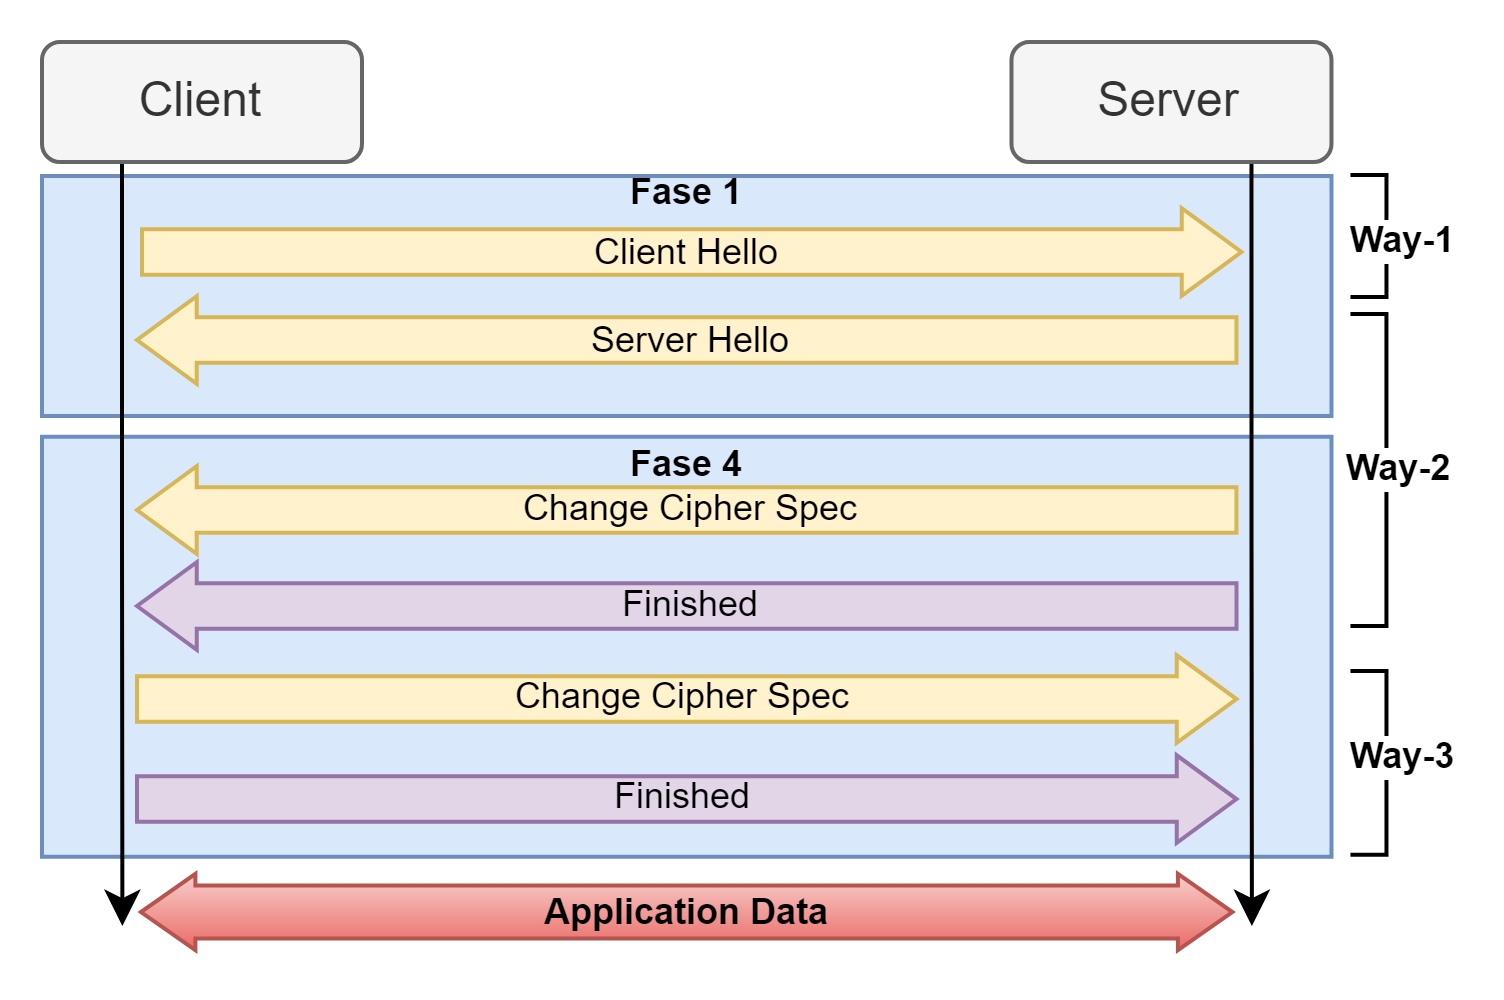
\includegraphics[width=\linewidth]{image/handshakeabbr.png}
    \caption{Handshake Abbreviato}
    \label{fig:handshakeabbr}
\end{figure}
%%%%%%%%%%%%%%%%%%%%%%%%%%%%%%%%%%%%%%%%
\section{Key Computation}
Nel protocollo TLS sono \textbf{utilizzati diversi segreti} e \textbf{nonces} \textbf{per la generazione delle chiavi di sessione }necessarie ai meccanismi di sicurezza concordati durante l’handshake. In particolare abbiamo:
\begin{itemize}
    \item \textbf{Nonces:} freschezza inserita sia da parte del client che da parte del server. Rispettivamente:
    \begin{itemize}
        \item \textbf{Client Nonce}: Inviata tramite \textbf{\textit{Client Hello}} (\cref{def:clienthello}), composta da timestamp e random value.
        \item \textbf{Server Nonce}: Inviata tramite \textbf{\textit{Server Hello}} (\cref{def:serverhello}), composta da timestamp e random value.
    \end{itemize}
    \item \textbf{Shared Secrets:} Usati "a catena" per generare le chiavi di sessione. Sono di due tipi:
    \begin{itemize}
        \item \textbf{Pre-Master Secret}
        \begin{definition}[Pre-Master Secret]\label{def:pms}
        Il PMS viene generato \textbf{una volta} per sessione. 
        \begin{itemize}
            \item Può essere \textbf{generato} dal \textbf{client} e \textbf{comunicato} al server con \textbf{RSA Key Transport} (\cref{fig:rsakeytrans}). In tal caso viene utilizzato solamente il \textbf{Client Key Exchange} message della fase 3 (\cref{prop:phase3}).
            \item Può essere \textbf{calcolato} tramite \textbf{DH Key Agreement} (\cref{def:dh}), utilizzando il \textbf{Server Key Exchange} della fase 2 (\cref{prop:phase2}) e il \textbf{Client Key Exchange} della fase 3.\\
            \begin{remark}
            Nel caso in cui venga usato \textbf{Fixed DH} (\cref{def:fixdh}) il valore del PMS è \textbf{costante} ad ogni nuova sessione, per una \textbf{fissata coppia client-server}
            \end{remark}
        \end{itemize}
        \end{definition}
        \item \textbf{Master Secret (MS)}: rigenerato ad ogni riavvio della sessione utilizzando il Pre Master Secret e le nonces del client e del server.
    \end{itemize}
    \item \textbf{Connection State Keys}
    \begin{definition}[Connection State Keys]
    chiavi di sessione rigenerate ad ogni riavvio e necessarie ai meccanismi di sicurezza negoziati durante l’handshake completo. Possono essere al più 6 chiavi, ovvero:
    \begin{itemize}
        \item \textbf{Due Chiavi} per la \textbf{criptazione simmetrica}
        \begin{itemize}
            \item $KC_C$: chiave per la criptazione \textbf{dal client al server}
            \item $KC_S$: chiave per la criptazione \textbf{dal server al client}
        \end{itemize}
        \item \textbf{Due chiavi} per il \textbf{controllo integrità}
         \begin{itemize}
            \item $KI_C$: chiave per la integrità \textbf{dal client al server}
            \item $KI_S$: chiave per la integrità \textbf{dal server al client}
        \end{itemize}
        \item \textbf{Due Initialization Vectors}, se necessari:
        \begin{itemize}
            \item $IV_C$: iv per la criptazione \textbf{dal client al server}
            \item $IV_S$:  iv per la criptazione \textbf{dal server al client}
        \end{itemize}
    \end{itemize}
    \end{definition}
\end{itemize}
Le \textbf{chiavi di sessione} vengono \textbf{rigenerate ad ogni riavvio} seguendo la strategia seguente:
\begin{definition}[Extract-then-Expand]\label{def:ete}
La strategia EtE consta di due fasi:
\begin{enumerate}
    \item \textbf{Extract}: viene \textbf{estratta} una chiave\textbf{ psuedo-random} \textbf{(il MS)} a partire da una\textbf{ chiave segreta} (il \textbf{PMS}) ed un \textbf{salt/seed} (le \textbf{nonces}). \\
    \begin{remark}
    Serve ad \textbf{aggiungere casualità nella generazione delle chiavi di sessione} rendendo l'MS casuale con distribuzione uniforme. Il PMS infatti potrebbe essere \textbf{biased} o addirittura \textbf{costante}.
    \end{remark}
    \item \textbf{Expand}: viene utilizzata una \textbf{PRF} per \textbf{espandere} arbitrariamente la \textbf{chiave pseudo-random generata nella fase precedente}. \\
    \begin{remark}
    Serve ad \textbf{estendere} un\textbf{ segreto limitato} alla quantità di materiale crittografico desiderata, ovvero al numero di chiavi di sessione necessarie.
    \end{remark}
\end{enumerate}
\end{definition}
La funzione PRF usata in \textit{\textbf{EtE}} può essere costruita utilizzando la costruzione HMAC (\cref{eq:hmac}) con una funzione \textbf{crypto hash} qualsiasi. Alcuni dei modi usati sono i seguenti:
\begin{itemize}
    \item Funzione di \textbf{Espansione Hash}:
    \[P_H(secret, label,seed)=HMAC_{H,secret}(A_1||A_0)||HMAC_{H,secret}(A_2||A_0)||\dots
    \]
    Dove $A_i=HMAC_{H,secret}(A_{i-1})$ e $A_0=ctx\_str||seed$. 
    \begin{remark}
    Questa costruzione \textbf{non è sicura} in quanto non fornisce garanzie sull'assenza di collisioni sul risultato prodotto. Ad esempio potremmo andare in contro a \textbf{short cycle problem} (\cref{def:shortcycle})
    \end{remark}
    \item \textbf{HMAC-Based Key Derivation Function}:
    \begin{definition}[HKDF]\label{def:hkdf}
    Costruzione sicura in quanto utilizza un contatore per evitare cicli.
    \[\text{HKDF}(secret,label,seed)=\text{HMAC}_{H,secret}(ctx\_str||0)||\text{HMAC}_{H,secret}(\cdot||1)||\dots\]
    \end{definition}
\end{itemize}
\begin{remark}
Con ctx\_str indichiamo una \textbf{context string}, ovvero una stringa formata da un testo arbitrario aggiuntivo e un seed.
Il suo contenuto è \textbf{esplicativo} del contesto nel quale stiamo calcolando la chiave e indica lo scopo della computazione, ad esempio:
\[PRF(master-secret, \textcolor{teal}{\text{\textbf{"client finished"}}}, \text{MD5}(\text{all handshake msg})|\text{SHA1}(\text{all handshake msg}))\]
\end{remark}
Con questi metodi si possono ottenere digest di lunghezza arbitraria e costruire le chiavi necessarie a TLS per operare correttamente ed utilizzare una chiave diversa per ogni servizio. Ogni versione del protocollo utilizza una propria PRF:
\begin{itemize}
    \item \textbf{SSL V3.0}: utilizza una PRF che non soddisfa le proprietà richieste.
    \item \textbf{TLS v1.0/v1.1}: usa $\text{PRF}(secret, lbl,seed)=P_{MD5}(secret,lvl,sd)\oplus P_{SHA-1}(secret,lbl,sd)$.
    \begin{remark}
    In queste versioni le funzioni hash erano hardcoded e l'uso di $P_H$ introduce problemi di short cycling, quindi è un metodo non sicuro. Inoltre, venne fatto lo xor di due funzioni crittografiche differenti, generando una costruzione senza nessuna prova matematica che fosse sicura.
    \end{remark}
    \item \textbf{TLS v1.2}: $P_H$ con funzioni hash negoziabili (default: SHA-256).
    \item \textbf{TLS v1.3}: Uso di $HKDF$ con funzione hash negoziabile (default: SHA-256).
\end{itemize}
\begin{figure}[h]
    \centering
    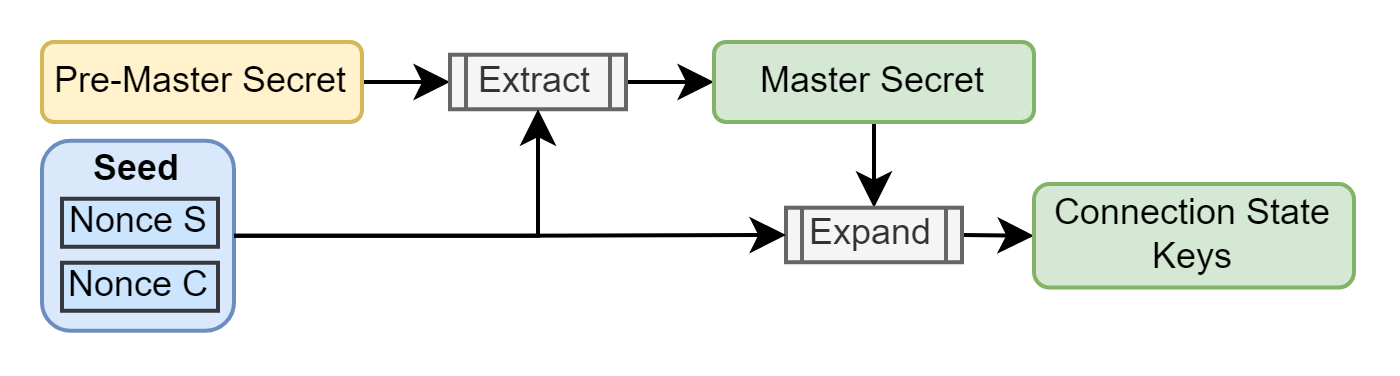
\includegraphics{image/kdf.png}
    \caption{KDF Scheme}
    \label{fig:kdf}
\end{figure}

\section{Other Minor Protocols}
Ci sono ulteriori protocolli minori necessari al funzionamento e alla gestione della sessione, come la gestione degli errori o cambio di stato della sessione.
\subsection{Change Chiper Spec Protocol}
\begin{definition}[Change Cipher-Spec Protocol]\label{def:changecipherprot}
Questo protocollo è definito come separato dall'Handshake Protocol per poter criptare \textbf{immediatamente} i messaggi successivi ad un \textit{Change Cipher Spec} message. Questi messaggi sono dei messaggi \textbf{vuoti} costituiti da un byte costante, di valore 0 o 1 per indicare il \textbf{cambio di stato} del \textbf{livello di sicurezza} della sessione TLS.
\end{definition} 
Inoltre:
\begin{theorem}[TLS Message Aggregation Principle]
Il \textbf{principio di aggregazione} dei messaggi TLS specifica che tutti i messaggi \textbf{provenienti da uno stesso livello o superiore} devono essere \textbf{aggregati} in un \textbf{unico TLS record}.\\
Inoltre, un TLS record deve essere \textbf{criptato per intero} e mai parzialmente.
\end{theorem}
Con tale soluzione i \textbf{\textit{finished message}} dell'handshake, poiché inviati \textbf{sempre dopo} i \textit{change cipher spec}, sono inviati sicuramente in un TLS record criptato \textbf{simmetricamente}.
\begin{figure}[h]
    \centering
    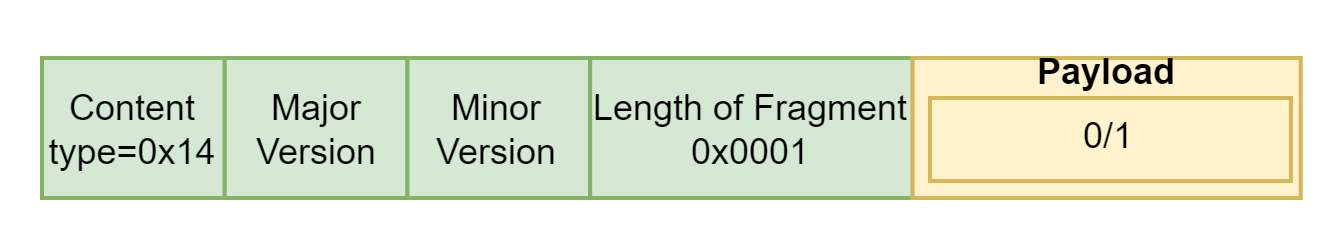
\includegraphics{image/changecipher.png}
    \caption{Change Cipher Spec Protocol Message}
    \label{fig:changecipher}
\end{figure}
\subsection{Alert Protocol}
\begin{definition}[Alert Protocol]\label{def:alertprot}
E' un protocollo che permette lo scambio  di \textbf{avvertimenti} tra client e server, al fine di segnalare avventimenti eccezionali e/o errori. A tale scopo vengono definiti messaggi speciali per comunicare e gestire tali casi.
\end{definition}
\begin{definition}[Alert Message Format]Il formato degli alert è il seguente:
\begin{itemize}
    \item \textbf{Alert Level} (1 byte) indica il livello di gravità che può essere:
    \begin{enumerate}
        \item \textbf{Warning:} la connessione/sicurezza può essere instabile.
        \item \textbf{Fatal:} la connessione/sicurezza può essere stata compromessa, oppure si è verificato un errore \textbf{non recuperabile} nell'esecuzione del protocollo.
    \end{enumerate}
    \item \textbf{Alert Description:} (1 byte) Descrive il significato dell'alert, ne esistono 23 diversi. Alcuni sono:
    \begin{itemize}
        \item \textbf{close\_notify:} Segnala la terminazione volontaria della connessione TLS.
        \item \textbf{unexpected\_message:} E' stato ricevuto un messaggio inappropriato.
        \item \textbf{bad\_record\_mac:} il MAC del TLS-Record non è corretto.
        \item \textbf{record\_overflow:} la lunghezza del TLS-Record è maggiore a quella massima consentita.
        \item \textbf{handshake\_failure:} impossibile negoziare un set accettabile di parametri di sicurezza dalle opzioni disponibili dichiarate dal client e/o dal server
        \item \textbf{bad\_certificate:} il certificato è corrotto e/o la firma è errata.
        \item \textbf{unsupported\_certificate:} il formato del certificato non è supportato.
        \item \textbf{certificate\_revoked:} il certificato è stato revocato.
        \item \textbf{certificate\_expired:} il certificato è scaduto.
    \end{itemize}
\end{itemize}
Questi messaggi sono \textbf{incapsulati} come \textbf{payload all’interno di TLS Record}. Nel caso in cui venga ricevuto un \textbf{fatal alert}, la \textbf{connessione} viene \textbf{terminata} e viene \textbf{impedito il riavvio} con gli \textbf{stessi parametri} di \textbf{sicurezza}.
\end{definition}
\begin{figure}[h]
    \centering
    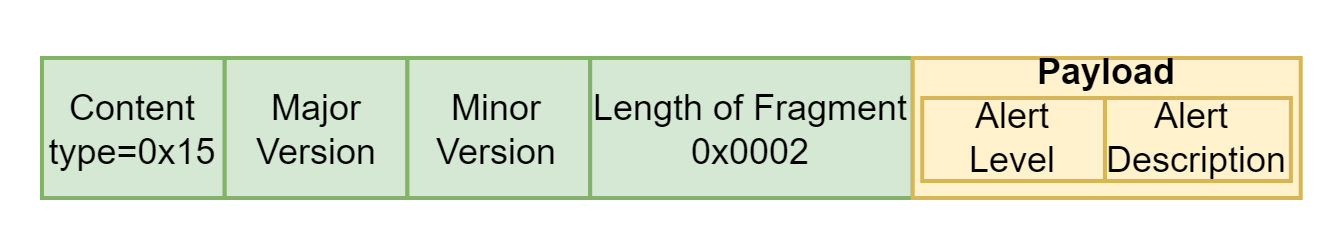
\includegraphics{image/tlsalert.png}
    \caption{Alert Protocol Message}
    \label{fig:tlsalert}
\end{figure}
\begin{remark}
Il warning di \textbf{close\_notify} viene utilizzato dal protocollo TLS per terminare la connessione in modo volontario da una delle due parti. Da questo momento in poi, una delle due parti specifica che \textbf{non} verranno più trasmessi ulteriori dati applicativi.
\end{remark}
Questo meccanismo permette di \textbf{distinguere} tra le \textbf{connessioni terminate volontariamente in modo sicuro}  e quelle \textbf{interrotte da cause esterne}, tra cui la \textbf{terminazione della} sottostante \textbf{connessione TCP}.
\subsection{Renegotiation}
La rinegoziazione è la possibilità di effettuare un handshake completo per una connessione TLS già esistente così da poter cambiare i parametri di sicurezza, come ad esempio il cipher suite utilizzato o autenticare una parte precedentemente non autenticata. Alcuni dettagli importanti sono:
\begin{definition}[Renegotiation (overview)]\label{def:renegotiation}
\begin{itemize}
    \item Viene \textbf{generato} un \textbf{nuovo Session ID} alla connessione TLS. In particolare, il \textbf{client genera un Client Hello con Session ID pari a 0} così che il \textbf{server utilizzi un Session ID differente dal precedente}.
    \item Oltre alle chiavi di sessione, vengono anche \textbf{rigenerati} il \textbf{pre-master secret ed il master secret}.
    \item L’\textbf{intero handshake per la rinegoziazione è criptato asimmetricamente} tramite \textbf{utilizzando il cipher suite in vigore}, a differenza del primo handshake, il quale è effettuato in chiaro.
    \item La\textbf{ rinegoziazione ha precedenza sui dati applicativi}. Eventuali dati generati dal server (il client è consapevole della rinegoziazione) durante l’esecuzione dell’handshake vengono bufferizzati localmente in chiaro in attesa che termini la rinegoziazione.
\end{itemize}
\end{definition}
Ne deriva che:
\begin{itemize}
    \item La \textbf{rinegoziazione non è distinguibile} dalle \textbf{negoziazione precedenti}, escluso il fatto che è criptato usando la precedente cipher suite. Inoltre, non sono legate crittograficamente tra loro.
    \item Una \textbf{transazione} effettuata a \textbf{livello applicativo} potrebbe essere \textbf{spezzata} in due parti dall'esecuzione di una rinegoziazione, comportando differenza nella sicurezza applicata alle due parti.
\end{itemize}
\begin{remark}
L'interruzione del livello applicativo genera delle vulnerabilità in TLS che \textbf{non} possono essere rilevate da cliene server.
\end{remark}

\section{DTLS}
Il protocollo DTLS è una versione del \textbf{protocollo TLS che viene trasportata tramite il protocollo UDP}. Le principali differenze con la versione tradizionale trasportata tramite il protocollo TCP sono:
\begin{definition}[DTLS Major Features]\label{def:dtls}
\begin{itemize}
    \item Viene utilizzato un \textbf{sequence number nell’header dei DTLS Record per il riordinamento} e dei \textbf{timeout per rilevare la perdita di datagrammi UDP}. 
    \begin{itemize}
        \item [$\rightarrow$]TLS assume la consegna in ordine dei segmenti TCP.
    \end{itemize}
    \item Sono aggiunti dei \textbf{meccanismi} di \textbf{frammentazione dei DTLS record}, così che possano essere \textbf{trasportati} in \textbf{un solo DTLS record}.
    \begin{itemize}
        \item [$\rightarrow$] In TLS possono essere generati dei TLS record di grandi dimensioni.
    \end{itemize}
    \item La \textbf{connessione} viene esplicitamente \textbf{delimitata dall’handshake} ed i \textbf{messaggi} di \textbf{close notify}.
     \begin{itemize}
        \item [$\rightarrow$] In TLS la connessione viene assunta dall’uso del sottostante protocollo TCP.
    \end{itemize}
\end{itemize}
\end{definition}
\section{Original Sin of TLS (up to v1.2)}
I servizi di integrity possono essere visti spesso come l'unico requisito da implementare, in quanto è generalmente importante prevenire lo spoofing (injection) o il tampering (modification) dei messaggi. In parole povere vale il seguente "motto": \textit{vedere ma non toccare}.\\
Allo stesso tempo, sappiamo che l'\textbf{encryption POTREBBE non garantire integrity}, a meno di usare \textbf{AEAD}\footnote{Come fatto in TLS v1.3} \cref{chap:aead}. I tre maggiori protocolli di sicurezza applicano i seguenti schemi di cifratura e autenticazione:
\begin{itemize}
    \item \textbf{TLS (up to v1.2):} MAC-then-Encrypt. Invio $ENC(Data, MAC(Data))$. Costruzione sbagliata, dimostrata e che porta ad attacchi chosen ciphertext. 
    \item \textbf{IPsec:} Encrypt-then-MAC. Invio $ENC(Data)|MAC(ENC(Data))$. L'unico modo giusto, ma \textit{AEAD} (\cref{chap:aead}) è meglio.
    \item \textbf{SSH:} Encrypt-then-MAC. Invio $ENC(Data)|MAC(Data)$. Nonostante possa essere visto come più efficiente in quanto encryption e integrity possono essere svolte in parallelo, è formalmente sbagliato in quanto il MAC da solo non protegge la confidentiality, ed essendo deterministico (il mac per uno stesso messaggio deve essere lo stesso per definizione) risulta facilmente attaccabile appena c'è un messaggio ripetuto.
\end{itemize}
\begin{remark}
Per le operazioni di decrittazione, è importante la dimensione dei pacchetti e, di riflesso, il padding usato. TSL specifica come definire il padding:
\end{remark}
\begin{definition}[TLS Padding]
Assumiamo che $L$ sia la dimensione di un blocco cifrato e che l'ultimo byte del blocco contenga proprio il valore di $L$. Se $L$ è la dimensione del blocco meno 1, allora viene inserito un byte di padding il cui valore è $00$. Se la dimensione è inferiore a quella di un blocco, allora come padding vengono inseriti tanti byte il cui valore è quello di $L$.\\
Se $L$ è pari alla dimensione del bloco e non sarebbe necessario padding, si crea un nuovo blocco composto da solo byte di padding.
\end{definition}
\begin{figure}[h]
    \centering
    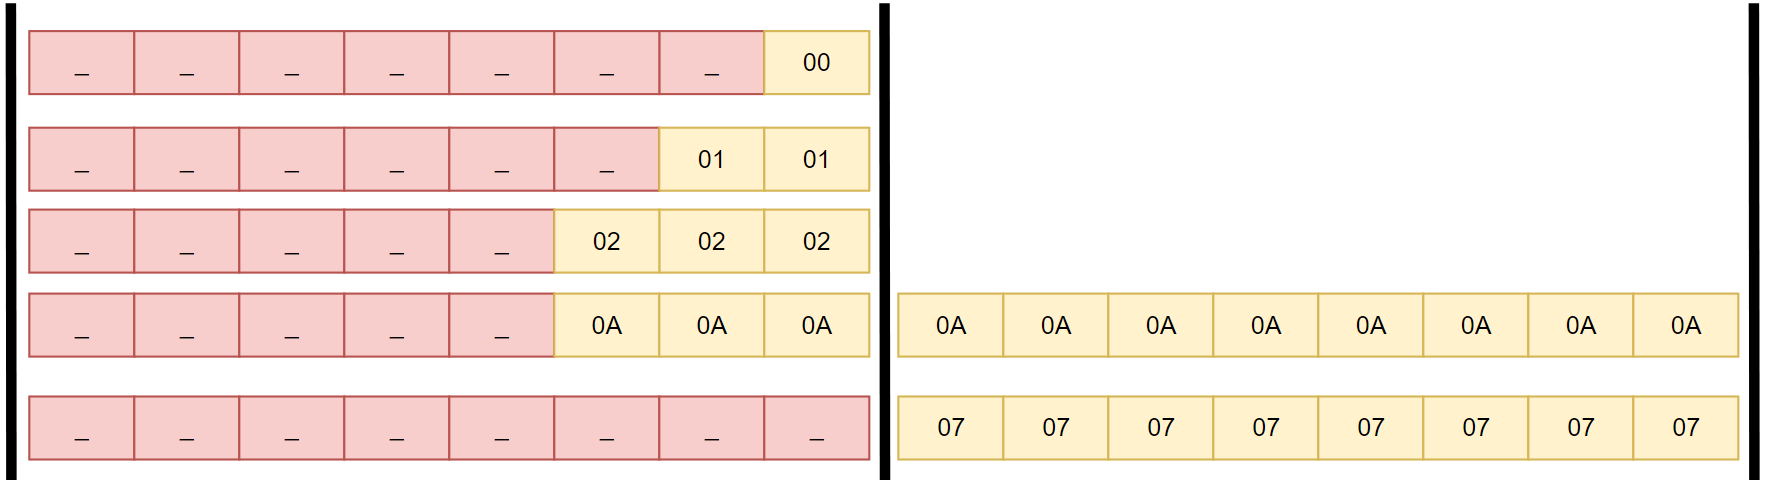
\includegraphics{image/tlspadding.png}
    \caption{TLS Padding}
    \label{fig:tlspadding}
\end{figure}
\subsection{Attacks to Encryption - Padding Oracle}
Nel \cref{chap:blkcipher} abbiamo visto i block cipher, che usano logiche "particolari" per cifrare i messaggi. TLS è fatto in modo di usare diversi cifratori e quindi gli attacchi sono \textit{relativi} allo specifico algoritmo usato. Tralasciamo algoritmi deboli e/o bucati, e concentriamoci su quelle cattive implementazioni che ci sono state.\\
Consideriamo TLS v1.0 e il meccanismo di decrittazione usato da CBC (\cref{def:cbcdec}). Riassumendo, il meccanismo si comporta nel seguente modo:
\begin{enumerate}
    \item \textbf{Applica decrittazione}: se il numero di byte \textbf{NON} è multiplo della dimensione del blocco ritorna un messaggio di alert \textbf{decryption\_failed}.
    \item \textbf{Rimuovi padding}: leggo dall'ultimo byte la lunghezza $L$ e rimuovo gli ultimi $L$ byte controllando che ogni blocco di padding sia uguale a $L$. Altrimenti ritorna un messaggio di alert: \textbf{decryption\_failed}.
    \item \textbf{Controlla MAC}: il controllo è fatto sul messaggio decifrato senza pad. Se fallisce ritorna un alert message: \textbf{Bad\_record\_mac}
\end{enumerate}
\begin{remark}
Il comportamento di error-signaling è tipico dei protocolli di rete, dove la \textbf{ragione dell'errore} viene sempre spiegata. 
\end{remark}
\begin{definition}[Padding Oracle Attack\footnotemark]\label{def:padoracle}
\footnotetext{\textsuperscript{\thefootnote}Modello di attacco valido \textbf{per ogni} block-cipher.}
Consideriamo un sistema che accetta messaggi cifrati e che usi un block-cipher per cifrare e decifrare i messaggi.\\
Supponiamo che il sistema possa rispondere in più modi quando riceve un messaggio sbagliato, ad esempio in 2 possibili modi (vedi TLS v1.0):
\begin{enumerate}
    \item \textbf{Decryption Failed:} Il \textbf{padding} è \textbf{sbagliato}.
    \item \textbf{Bad-MAC:} Il \textbf{padding} è \textbf{giusto} e il \textbf{server} è \textbf{arrivato} al \textbf{terzo check}.
\end{enumerate}
Supponiamo che l'attaccante \textbf{disponga di un ciphertext} $C$ (ad esempio in risposta di una challenge) e che sia in grado di \textbf{forgiare un ciphertext} $C'$ che inoltra al sistema, la cui probabilità di essere valido è trascurabile\footnotemark.\\
Sapendo il modo con cui questo decrypta il messaggio e restituisce il codice d'errore l'attaccante ha a disposizione un \textbf{oracle} che, dato un messaggio cifrato in ingresso, è in grado di fornire informazioni sul plaintext.
\footnotetext{\textsuperscript{\thefootnote}Anche se i ciphertext sono corretti con \textbf{probabilità} \textbf{"negligible"}, l'errore può essere controllato a prescindere.}
\end{definition}
\begin{remark}
Non è necessario che il sistema risponda con un codice esplicito di errore. Spesso differenze nel tempo di elaborazione e nel comportamento che assume il sistema possono essere un indicatore per un attaccante in grado di intercettare questi dettagli.
\end{remark}
\begin{example}[ Padding Oracle in TLS v1.0]\label{exam:padoracle}\hfill\\
Consideriamo lo scenario di TLS e, per semplicità, supponiamo che stia usando CBC (\cref{fig:cbcdec}) e che l'attaccante disponga di un ciphertext formato da $c[0],c[1]$ e del relativo $IV$.\\ 
Per come funziona CBC in decryption abbiamo che:
\begin{equation*}
    \begin{aligned}
    m[0] &= {PRP}^{-1}_k(c[0])\oplus{IV}\\
    m[1] &= {PRP}^{-1}_k(c[1])\oplus{c[0]}
    \end{aligned}
\end{equation*}
Poiché tale relazione è lineare nello xor, una modifica nell'i-esimo byte dell'IV implica una modifica nell'i-esimo byte di m[0] e, analogamente, una modifica nell'i-esimo byte di c[0] causa una modifica nell'i-esimo byte di c[1].\\
Senza perdita di generalità supponiamo di voler conoscere $m[1]$\footnote{se avessimo voluto conoscere $c[0]$ avremmo lavorato con l'$IV$.}, quindi \textbf{supponiamo di modificare l'ultimo byte di $c[0]$} con un carattere da $v$ da noi scelto in modo tale che:
\[c[0](n) = c[0](n)\oplus{v}\oplus{0\times00}\]
Dove $0\times00$ è il padding che ipotizziamo possa essere stato fatto in quanto stiamo indovinando l'ultimo carattere e, pertanto, potrebbe non esser stato necessario paddarlo.\\
Inviando questo messaggio all'oracolo riceveremo, nella maggior parte dei casi, un messaggio di errore:
\begin{enumerate}
    \item \textbf{Decryption Failed}: non resta che provare un nuovo carattere $v$ poiché non abbiamo indovinato l'ultimo carattere.
    \item \textbf{Bad-MAC}: allora il messaggio decifrato sarà $m[1] = xx\,xx\,xx\,xx\,|0\times00$. Tale messaggio produrrà un MAC diverso ma a noi non importa perché abbiamo scoperto il padding che era stato fatto su $m[1]$ e il valore del suo ultimo byte, ovvero: $m[1]=xx\,xx\,xx\,xx\,v$.
\end{enumerate}
Dal caso due capiamo che l'attaccante è ora a conoscenza dell'ultimo carattere di $m[1]$ e ora può iterare facendo brute-force su tutti i byte rimanenti, aumentando di 1 il valore del padding così da non alterare la dimensione del blocco che verrà controllato. In questo modo il sistema attaccato, controllando l'ultimo byte contenente la lunghezza del messaggio, arriverà sempre al terzo check. 
\begin{remark}[Complessità dell'Attacco]
La complessità dell'attacco è $\leq{L}$, dove $L$ è la lunghezza del blocco da decifrare. Con 8 un blocco da byte avremmo al più $(2^8)*8$ per decriptare un solo block.
\end{remark}
\begin{remark}[Ricorsione per determinare il Padding]
E' possibile determinare il padding fatto sul blocco da decifrare partendo dal modificare uno alla volta i primi $k$-byte dell'IV relativo finché non otteniamo un \textbf{DECRYPTION\_FAILED}. Allora il padding fatto sarà $n-k$ e possiamo provare l'attacco.
\end{remark}
\end{example}
\begin{figure}[ht]
    \centering
    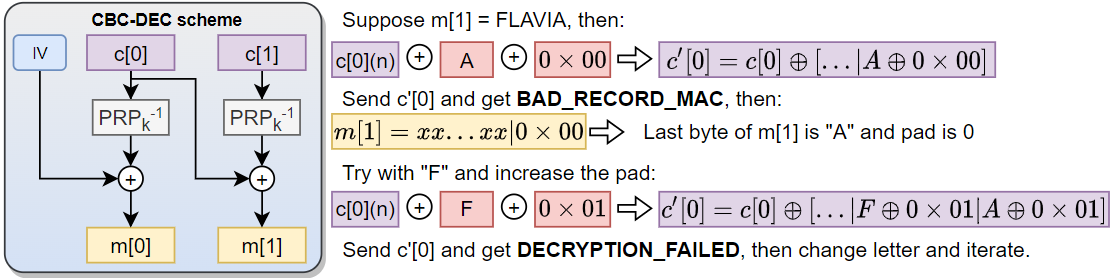
\includegraphics[width=\linewidth]{image/padoracle.png}
    \caption{Padding Oracle}
    \label{fig:padoracle}
\end{figure}
\subsection{Solutions of next versions and Final Considerations}Dall'esempio \ref{exam:padoracle} capiamo che MAC-than-Encrypt \textbf{NON E' MAI LA SCELTA MIGLIORE}, in quanto per proteggersi da un padding oracle sarebbe bastato autenticare il testo cifrato, così da bloccare ogni possibile modifica ad esso.\\
TLS 1.0 infatti venne patchato, selezionando come ritorno in caso di errore sempre e solo \textbf{BAD\_MAC}, soluzione poi standardizzata da TLS 1.1 e cambiata in \textbf{TLS v1.2}, dove se il \textbf{padding falliva}, il \textbf{MAC} era \textbf{validato in OGNI caso}.
Questo perché fino alla v1.1 tramite side-channels era comunque possibile capire grazie al tempo di risposta del server in quale fase ci fosse stato il fallimento in quanto più tempo di risposta implica che l'errore è avvenuto in una fase successiva.\\
\begin{corollary}[Problem with TLS v1.2 workaround]
Validando il MAC in ogni caso, sorge il problema di \textbf{non sapere più quale dato viene validato}, poiché se il padding-check fallisce non abbiamo modo di conoscere la dimensione del messaggio rispetto a quella del padding. TLS v1.2 usava l'\textbf{intero messaggio} per convalidare, ma questo implicava l'uso di più dati e più tempo per calcolare l'HMAC.
\end{corollary}
\begin{remark}
L'unico modo per patchare definitivamente TLS fu quello di rimuovere ogni forma di combinazione di ENC e MAC e di usare AEAD.
\end{remark}
\begin{proposition}[Praticità dell'Attacco]
Un padding oracle potrebbe non essere applicabile in ogni scenario della realtà, in quanto TLS appena rileva un errore chiude la connessione e bisogna ricominciare daccapo. Tuttavia, resta uno strumento molto forte nelle mani di un hacker.
\end{proposition}
Nel 2003 è stato dimostrato che l'attacco è realizzabile su protocollo IMAP, in quanto i client IMAP fanno periodicamente login ogni 5 minuti, trasmettendo le credenziali che vengono inviate \textbf{sempre con lo stesso format}. Facendo un DNS spoofing (MITM) è stato possibile effettuare un CCA, ottimizzando con strategie dictionary attack per scoprire le password.
\section{Major Vulnerabilities}
Una delle più grandi falle in TLS 1.0 fu la \textbf{scelta} di implementare hardcoded gli algoritmi di cifratura, compromettendone la resistenza \textit{a lungo termine}.\\
Uno degli algoritmi implementati era CBC, il quale soffre di un problema di \textit{IV-prediction}, Infatti per operare la cifratura di una serie di messaggi, soltanto il primo IV del primo gruppo di blocchi veniva generato "on-the-fly", perché per gli altri gruppi veniva usato l'ultimo cipherblock del gruppo precedente.
\begin{remark}
Se l'IV dipende dal blocco precedente, nonostante abbiamo la sicurezza semantica (IND-CPA), un attaccante può predire l'IV del prossimo processo di encryption e arrivare al plaintext.
\end{remark}
\begin{figure}[ht]
    \centering
    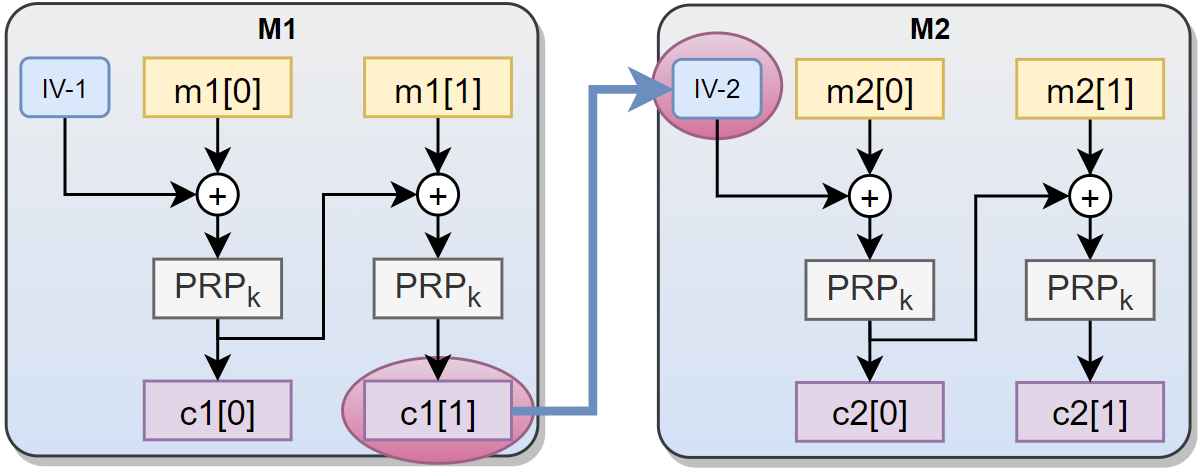
\includegraphics[width=\linewidth]{image/ivpred.png}
    \caption{Last ciphertext-block of M1 used as IV for M2}
    \label{fig:ivpred}
\end{figure}
Lo schema di attacco per un IV prevedibile è allora il seguente:
\begin{definition}[IV Prediction Attack]\label{def:ivpredatk}
Supponiamo di sapere che l'i-esima porzione di m, $m[i]$, contenga una password e supponiamo per semplicità che la password possa essere $A$ o $B$. Consideriamo lo schema di encryption di CBC (\cref{def:cbcenc}). Poiché \textbf{CBC è semantic secure}, non è possibile usare un CPA, ma è possibile osservare $c[i-1]$.\\
Sia $X$ l'IV predetto, allora, forgiamo un ciphertext tale che:
\[c^{'}[i-1]=X\oplus{c[i-1]}\oplus{Guessed\_PWD}\]
Se l'IV è stato predetto correttamente, allora basterà chiedere al sistema di cifrare per noi $m[i]$ con IV pari a  $c^{'}[i-1]$. \\
Se $c^{'}[i-1]=c[i]$, allora abbiamo individuato la password. Altrimenti dobbiamo provare l'altra password.
\end{definition}
\begin{remark}
Inizialmente si pensava che l'attacco fosse impossibile da realizzare davvero, ma la vulnerabilità venne exploitata davvero tramite le moderne tecnologie, come HTML5. Ad esempio, tramite l'inserimento forzato di chosen plaintext facendo girare codice direttamente sul browser dell'utente.
\end{remark}
\subsection{BEAST Attack: Chosen Boundary Attack}
Consideriamo i cookie di un servizio on-line. Questi oggetti contengono in locale delle informazioni utili alle web-app per \textit{velocizzare} l'utilizzo delle stesse, al fine di portare un vantaggio all'utente. Ad esempio sono utili per effettuare un \textit{"login veloce"}, in quanto il browser può auto-completare i campi e-mail e password di un form.\\
Tuttavia, è stato provato che è possibile decifrare i cookie di un browser e la complessità è lineare con la loro lunghezza. Questo lavoro è stato provato da Duong e Rizzo, nell'attacco BEAST\footnote{\href{https://bug665814.bmoattachments.org/attachment.cgi?id=540839}{BEAST}}.

\begin{definition}[Chosen Boundary Attack]\label{def:beastatk}
Supponiamo che un cookie contenga nell'ultimo blocco la password di un utente, supponiamo di sapere il punto in cui la password comincia, per semplicità\footnotemark. Abbiamo allora a disposizione: $IV=c[i-1]$, $c[i]=Enc_k(c[i-1]\oplus{P[i]})$ e vogliamo indovinare $P[i]$.
\begin{enumerate}
    \item Aggiungiamo davanti alla stringa da attaccare una stringa da noi scelta, per fare in modo di allineare \textbf{il primo carattere della pwd} all'ultimo byte di blocco considerato.
    \item Lanciamo un brute-force attack, costringendo la vittima a lavorare come un encryption oracle. Il chosen plaintext che vogliamo inviare ha la struttura seguente:
    \begin{equation}\label{eq:beastcpa}
        P[i+1] = c[i]\oplus{Guess}\oplus{c[i-1]}
    \end{equation}
    In questo modo quando quello che verrà cifrato sarà esattamente la stessa cosa che era stata cifrata all'inizio, ovvero: 
    \begin{equation}
    \begin{aligned}
        c[i+1]&=Enc_k(c[i]\oplus{P[i+1]})\\
        &=Enc_k(c[i]\oplus{c[i]\oplus{Guess}\oplus{c[i-1]}})\\
        &=Enc_k(\oplus{Guess}\oplus{c[i-1]})
    \end{aligned}
\end{equation}
    \item Se $c[i+1]=c[i]$, allora significa che il \textbf{guess} è il plaintext cercato. Shiftando un carattere alla volta e modificando la la stringa aggiunta all'inizio, possiamo far entrare un carattere alla volta nel blocco da decifrare e scoprire tutta la password.
\end{enumerate}
\footnotetext{\textsuperscript{\thefootnote}Altrimenti avremmo solo bisogno di più tempo per decifrare la password.}
\end{definition}
\begin{figure}[h]
    \centering
    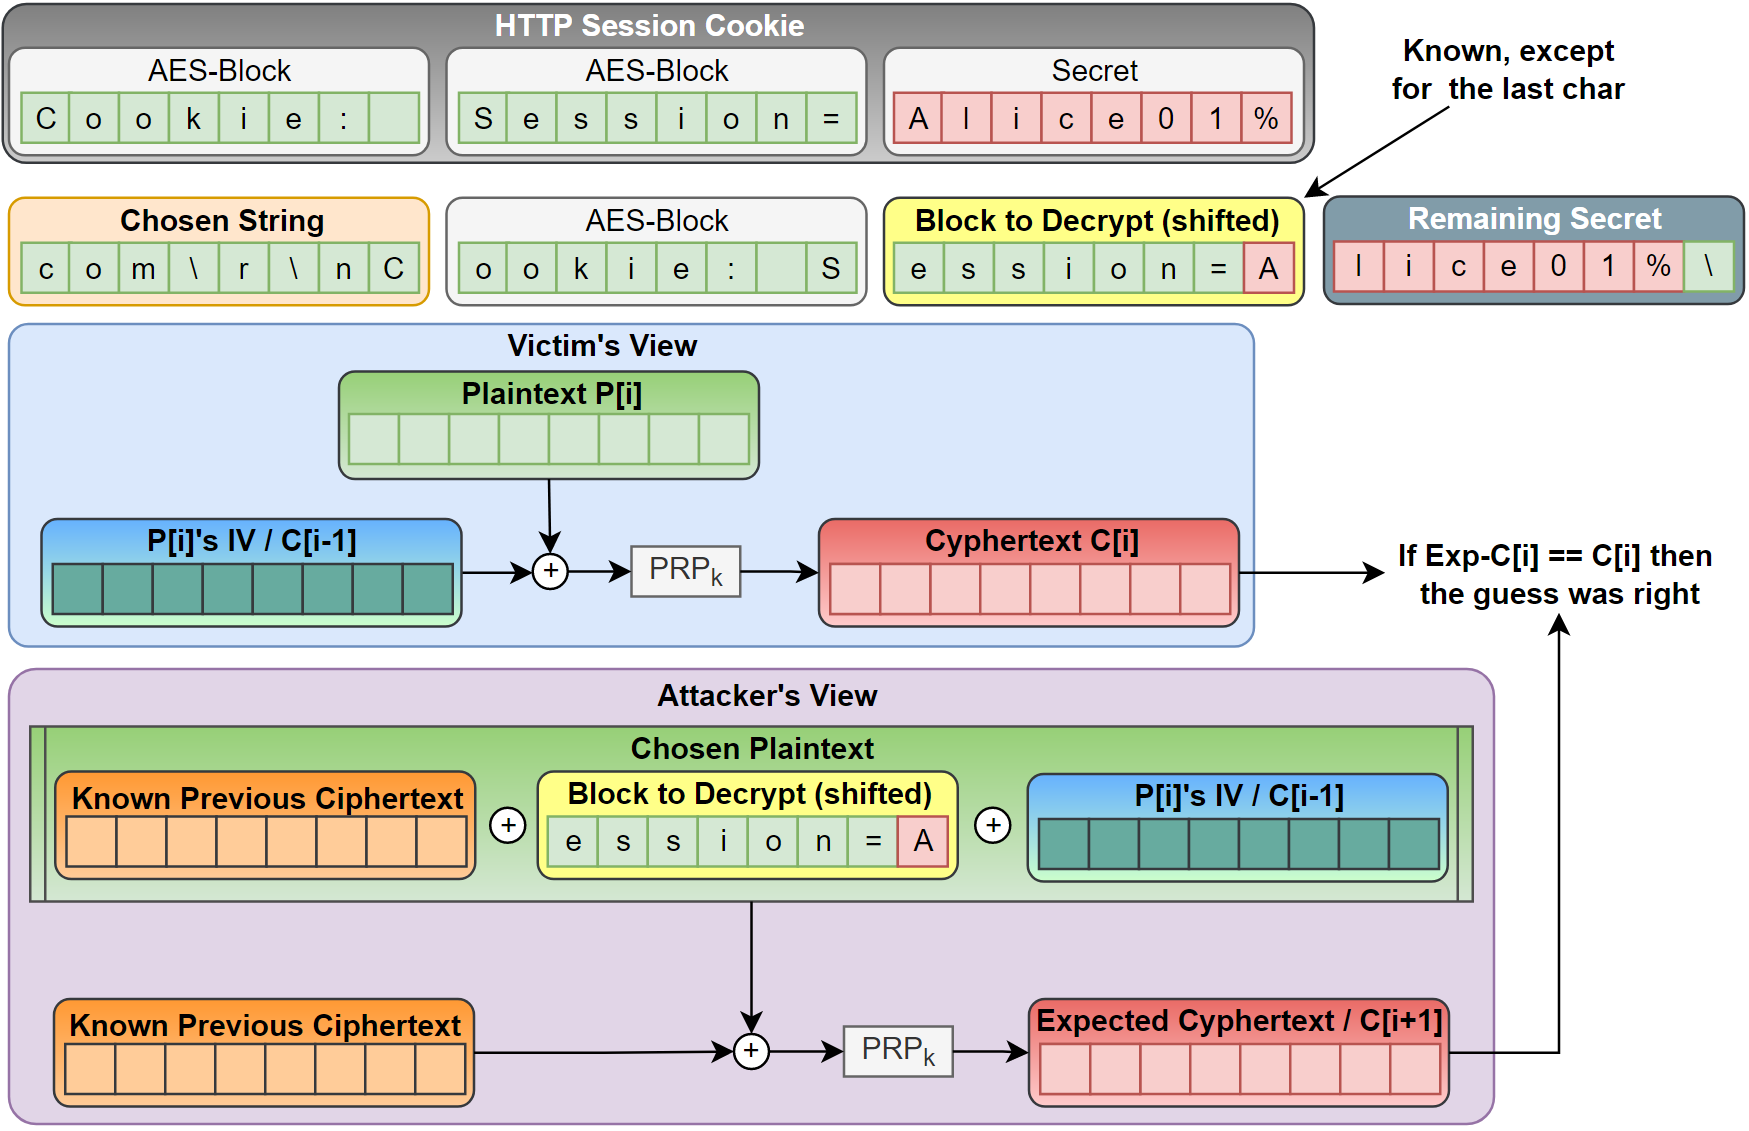
\includegraphics[width=\linewidth]{image/beast.png}
    \caption{BEAST Attack}
    \label{fig:beast}
\end{figure}
\subsection{CRIME Attack: Compression after Encryption leakeage}
Nel 2012, Duong e Rizzo dimostrarono che la compressione messa in atto da TLS portava ad un leak di informazioni riguardo il plaintext. Saltò fuori che in realtà il problema è intrinseco a qualsiasi sistema di compressione. Infatti:
\begin{example}[ Compression Size Leak]
Consideriamo una password di 6 byte: $AAAABC$. Applichiamo \textbf{Compress-than-Encrypt}, producendo prima $4ABC$ e poi $X\&\%\$$.
\begin{remark}
La lunghezza della password è passata da 6 a 4B.
\end{remark}
Consideriamo un'altra password da 6 byte, la cui entropia è maggiore: $ABCDEF$. Poiché l'entropia è massima, la compressione produrrà: $ABCDEF$ e l'encryption $\&\$\text{£A£}\$$.
\begin{remark}
La lunghezza della password è rimasta a 6B.
\end{remark}
\end{example}
Un attaccante ha ora una chance, unendo il size-leaking con un plaintext-injection. 
\begin{definition}[Compression with CPA]\label{def:compcpa}
Supponiamo di voler indovinare la password di un utente e \textbf{supponiamo di conoscere la dimensione} del \textbf{pacchetto compresso e cifrato}. Allore:
\begin{itemize}
    \item Supponiamo di poter intercettare il messaggio contenente la password trasmessa e di poter modificare il messaggio trasmesso, ma di non poterlo leggere.
    \item Appendiamo un plaintext composto da lettere tutte uguali\footnotemark all'inizio del testo sconosciuto.
    \item Il messaggio modificato verrà compresso e cifrato. Possono succedere 2 cose:
    \begin{enumerate}
        \item \textbf{$len(c'[i])=len(c[i])$:} La compressione non è stata utile perché l'entropia era troppo alta.
        \item \textbf{$len(c'[i])<len(c[i])$:} Il testo che abbiamo aggiunto ha ridotto l'entropia ed è stato compresso.
    \end{enumerate}
\end{itemize}
Se la lunghezza è stata ridotta, significa che la nostra aggiunta era \textbf{UGUALE} (almeno) alla prima lettera della password. 
\footnotetext{\textsuperscript{\thefootnote}set di $n$ lettere tutte uguali: $AAA$}
\end{definition}
\begin{remark}
Non potremmo comunque sapere tutta la password in questo modo, soltanto la prima o le prime lettere, se dovessere essere uguali. 
\end{remark}
Lo schema descritto venne adottato nell'attacco \textbf{CRIME}\footnote{Compression Ratio Info-Leak Made Easy}, sempre ad opera di Duong e Rizzo nel 2012. Riutilizzando gli stessi tool di BEAST, riuscirono a fare plain-text injection per sfruttare una vulnerabilità di \textit{\textbf{DEFLATE}}, un algoritmo di compressione basato sulla codifica \textit{\textbf{Huffman}}\footnote{\href{https://it.wikipedia.org/wiki/Codifica_di_Huffman}{Huffman Encoding}} e su \textbf{\textit{LZ77}}, una politica di compressione che \textbf{sostituisce 3 o più caratteri ripetuti} in una stringa con una \textbf{coppia $(\text{Offset}, \text{Size})$} che costituisce un puntatore ad un punto precedente della stringa.
\begin{example}[ LZ77]Consideriamo la seguente stringa:
\textit{Giuseppe \textcolor{orange}{Bianchi} and Marco \textcolor{orange}{Bianchi}ni}\\
Questa viene compressa in: \textit{Giuseppe \textcolor{blue}{Bianchi} and Marco \textcolor{blue}{(-18,7)}ni}.
\end{example}
L'idea dello schema di CRIME è quindi il seguente:
\begin{definition}[CRIME]\label{def:crime}
Supponiamo di conoscere un testo generato da un utente, composto da una parte \textbf{conosciuta}, l'\textbf{"Header"} e una parte \textbf{non nota}, il \textbf{Secret}. Ad esempio: \[[Authentication Token: passwd = alice\%01]\]
\begin{enumerate}
    \item Creiamo multipli messaggi composti da: 
    \[Att\_input + [header + secret]\]
    \item Inviamo e osserviamo il risultato della \textbf{compress-than-enc}:
    \[\text{Len}(Enc(Compress(Att\_input + [header + secret])))\]
\end{enumerate}
\end{definition}
\begin{figure}[h]
    \centering
    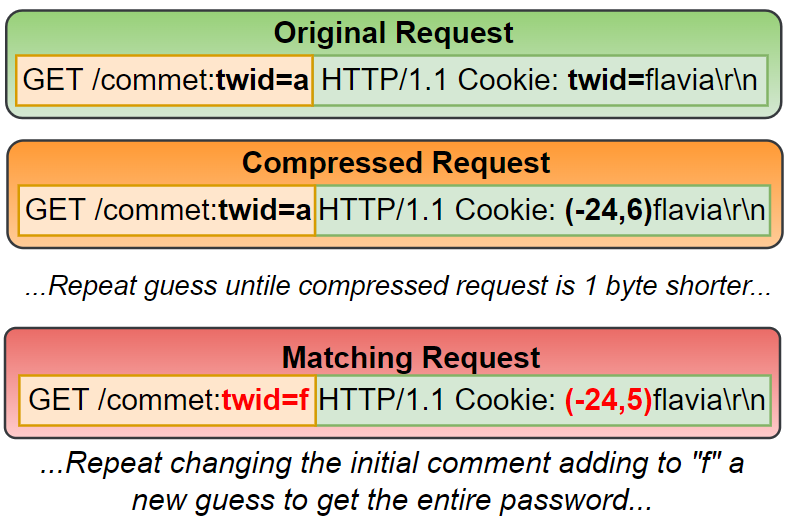
\includegraphics[width=0.7\textwidth]{image/crime.png}
    \caption{CRIME example for auth token in HTTP session}
    \label{fig:crime}
\end{figure}
\begin{remark}
In realtà  ci sono altri dettagli tecnici che andrebbero sviscerati, ma che non sono stati trattati, come il fatto che la compressione lavora sui singoli bit e non su byte, oppure che abbiamo completamente trascurato la codifica usata.\\
E' interessante osservare anche che l'attacco venne fatto su due protocolli diversi, TLS e SPDY (considerato HTTP2.0) e che il meccanismo è agnostico al sistema di cifratura.
\end{remark}
\subsection{Downgrade Attack}
Il downgrade attack si basa su potenziali vulnerabilità \textbf{nella fase 1} dell'handshake protocol. Si tratta di un MITM con l'obiettivo di modificare la versione in uso di TLS tra client e server, affinché sia possibile sfruttare ulteriori falle.\\
Idealmente l'attacco è possibile in quanto per retrocompatibilità, stabilità ed affidabilità, diverse sistemi non vengono aggiornati a versioni recenti dei protocolli perché troppo costoso in termini di risorse (temporali ed economiche). Vediamone le caratteristiche:
\begin{definition}[Downgrade Attack]\label{def:tlsdown}
Il MITM sfrutta l'assenza di message authentication della fase 1, per modificare il contenuto di \textbf{Client Hello} e \textbf{Server Hello}. In particolare, viene cambiato il campo della versione del protocollo, con una arbitrariamente scelta dall'attaccante.\\
Se la versione scelta è supportata dal server, allora questo risponde con un server hello con la versione modificata.
\end{definition}
\begin{figure}[h]
    \centering
    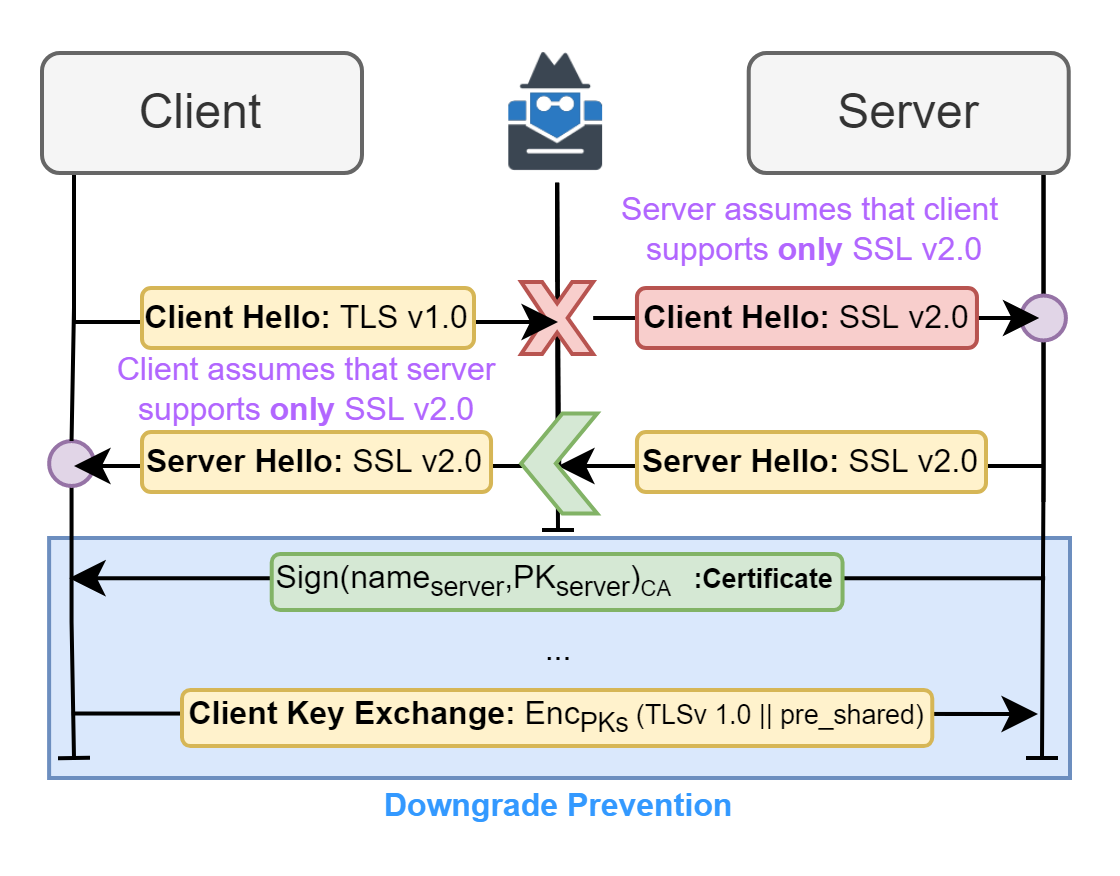
\includegraphics[width=0.7\textwidth]{image/tlsdown.png}
    \caption{Downgrade Attack and Prevention}
    \label{fig:tlsdown}
\end{figure}
\begin{proposition}[Downgrade Prevention]
Durante la fase 2 e 3 un downgrade attack viene intercettanto in quanto:
\begin{itemize}
    \item Il \textbf{certificate message} inviato dal server, firmato dalla CA, permette di \textbf{comunicare} in maniera \textbf{sicura} la chiave pubblica del \textbf{server}, con la quale il client cripterà asimmetricamente il contenuto dei suoi messaggi.\\
    \begin{remark}
    Questo avviene perché il certificato \textbf{non} può essere modificato dall'attaccante senza che non venga rilevato dal client, \textbf{impedendo} la \textbf{sostituzione} delle chiavi.
    \end{remark}
    \item Il \textbf{client key exchange} inviato dal client contiene al suo interno la versione di protocollo usata e dichiarata nel Client Hello. Il server può allora rilevare modifiche effetuate dall'attaccante.\\
    \begin{remark}
    L'attaccante non può neanche decriptare la pre-master secret inclusa nel messaggio, per cui non può inferire nulla sulle future chiavi di sessione.
    \end{remark}
\end{itemize}
\end{proposition}
\begin{remark}
Si noti che il \textbf{Certificate message non} è \textbf{obbligatorio} e che il \textbf{Client Key Exchange} potrebbe essere ut\textbf{ilizzato solamente} per inviare la \textbf{pre-master secret al server}, ovvero \textbf{non includere la versione TLS} dichiarata dal client, rendendo di fatto il Downgrade attack realizzabile su alcune istanze TLS.
\end{remark}
\subsection{Truncation Attack}
Il \textbf{truncation attack} si basa sulla vulnerabilità a \textbf{DoS Attacks}\footnote{Denial of Service} del sottostante protocollo TCP che si occupa di trasportare il \textbf{protocollo TLS}. In particolare, l'attacco è caratterizzato nel seguente modo:
\begin{itemize}
    \item \textbf{Obiettivo:} \textbf{Terminare} una \textbf{connessione TLS} tra client e server
    \item \textbf{Abilità:} inviare \textbf{segmenti TCP contraffatti} (\textbf{spoofing attack})
\end{itemize}
L'attaccante può inviare semgneti TCP-FIN contraffatti per far terminare la connessione TCP sottostante che trasporta il protocollo TCP.\\
Due possibili correzioni per proteggere delle applicazioni non consapevoli dei \textbf{protocolli sottostanti utilizzati} si basano sull'uso della \textbf{tecnica} del \textbf{tunnelling}, e sono:
\begin{theorem}[TCP over TLS over TCP]
la \textbf{connessione TCP utilizzata dall'applicazione} viene \textbf{trasportata} all'interno del protocollo \textbf{TLS}, a sua volta \textbf{trasportato} da una \textbf{seconda istanza TCP}. L'attacco risulta perciò trasparente all'applicazione, in quanto viene interrotta la seconda istanza TCP ma non quella utilizzata dall'applicazione stessa.
\end{theorem}
\begin{remark}
L’uso di una doppia connessione TCP degradare le prestazioni della connessione complessiva in quanto gli algoritmi di congestion control delle diverse istanze del protocollo possono andare in conflitto tra loro. Inoltre, se la soluzione prevede anche differenti connessioni TCP tra i nodi intermedi della comunicazione, tale problematica viene amplificata.
\end{remark}
\begin{theorem}[TCP over DTLS over UDP]
la \textbf{connessione TCP utilizzata dall'applicazione} viene \textbf{trasportata} all'interno del protocollo \textbf{DTLS}, a sua volta \textbf{trasportato} da una \textbf{seconda istanza UDP}. L'attacco viene vanificato dall'assenza di una connessione reale in quanto il trasportatore finale è il protocollo UDP.
\end{theorem}
\begin{remark}
L’uso del protocollo UDP rende inaffidabile la consegna dei segmenti UDP, sebbene permetta di evitare conflitti tra le varie istanze del protocollo e migliorare quindi le performance.
\end{remark}
\begin{remark}
Il \textbf{protocollo TLS attenua gli effetti che il Truncation attack} può generare \textbf{utilizzando} i \textbf{warning} alert di \textbf{Close Notify}, così che le parti possano \textbf{distinguere} tra \textbf{connessioni TLS terminate legittimamente} e \textbf{connessioni TLS terminate per cause esterne}. Resta comunque debole a tale attacco.
\end{remark}
\subsection{Renegotiation Attack}
Il Renegotiation attack si basa sulle vulnerabilità offerte dalla rinegoziazione TLS \cref{def:renegotiation}. L'attacco è caratterizzato nel seguente modo:
\begin{itemize}
    \item \textbf{Obiettivo:} ottenere \textbf{informazioni} sui \textbf{dati applicativi} protetti tramite TLS.
    \item \textbf{Abilità:} è in grado di \textbf{Innescare} una \textbf{rinegoziazione} (\textbf{MITM}), effettuare \textbf{plaintext injection attack} al \textbf{server} (\textbf{CPA)}).
\end{itemize}
\begin{definition}[Renegotiation Attack]\label{def:renegoatk}
Assumiamo che:
\begin{enumerate}\setcounter{enumi}{-1}
    \item Se il client invia un \textbf{client hello} \textbf{prima} dell'attaccante, quest'ultimo lo \textbf{intercetta} e lo \textbf{ritarda} fino al \textbf{termine} del \textbf{plaintext injection}.
    \item L'\textbf{attaccante} avvia un \textbf{handshake} a nome del client, sfruttando l'assenza di cipher suite e l'opzionalità dell'autenticazione del client.
    \item L'\textbf{attaccante} effettua (preable) \textbf{plaintext injection} sul server, inviando dati malevoli.
    \item L'\textbf{attaccante permette} al \textbf{client} di effettuare l'\textbf{handshake} e di \textbf{inviare i propri dati applicativi}, che verranno accodati a quelli precedentemente inviati dall'attaccante.
    \item L'\textbf{attaccante} visualizza l'\textbf{esito} dell'attacco\footnotemark
\end{enumerate}
\footnotetext{\textsuperscript{\thefootnote}Varia in funzione dell'applicazione e dell'attacco stesso.}
\end{definition}
\begin{figure}[h]
    \centering
    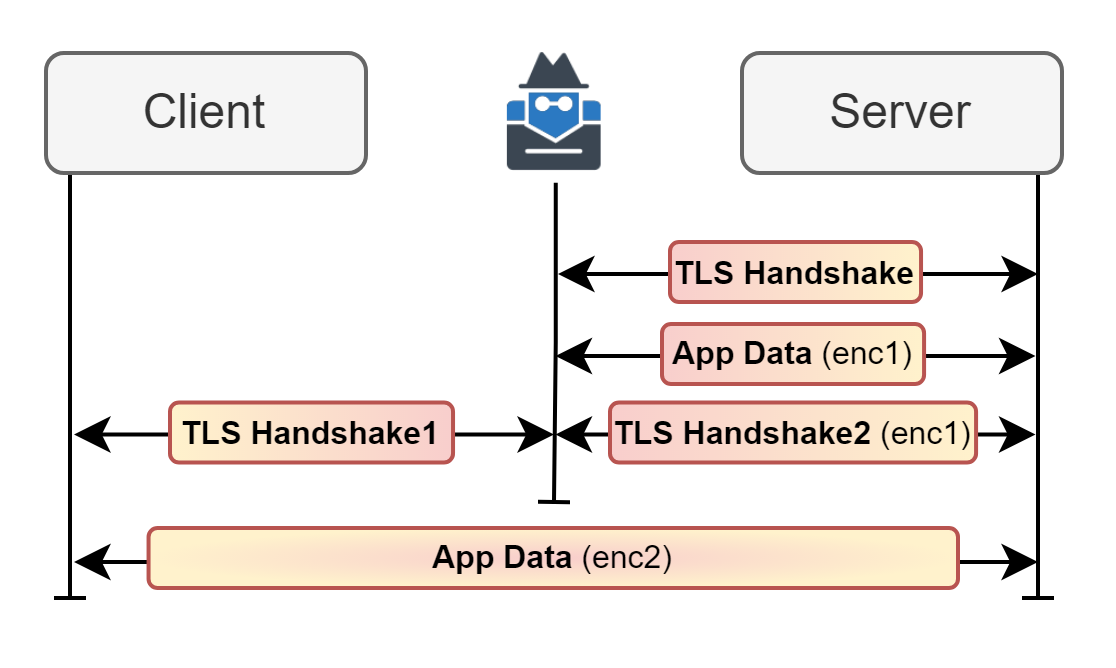
\includegraphics[width=0.7\textwidth]{image/renegoatk.png}
    \caption{Renegotiation Attack}
    \label{fig:renegoatk}
\end{figure}
Il renegotiation attack è stato corretto in TLS v1.2 con la \textbf{TLS Renegotiation Extension}, che prevede l'aggiunta di un \textbf{campo reneg} all'interno del \textbf{client hello}, utilizzata nel seguente modo.
\begin{enumerate}
    \item Nella \textbf{prima negoziazione:} il campo contiene un byte pari a 0 per indicare che è il \textbf{primo handshake completo} per la corrente sessione TLS.
    \item Nelle \textbf{rinegoziazioni:} contiene l'ultimo \textbf{finished message} del \textbf{precedente handshake}, così da indicare implicitamente l'\textbf{avvenimento di una rinegoziazione} e \textbf{legare crittograficamente} tra loro le \textbf{rinegoziazioni successive}. Ciò permette di \textbf{rilevare} l'avvenimento di un attacco.
\end{enumerate}
\begin{remark}
La rinegoziazione è stata \textbf{disabilitata} in TLS v1.3 poiché considerata troppo vulnerabile.
\end{remark}
\section{TLS v1.3}
La versione più recente e sicura del protocollo TLS presenta delle differenze sostanziali, tant'è che potremmo definirla una 2.0. Le principali sono:
\begin{theorem}[TLS v1.3 "Changelog"]\label{thm:tls13}
\begin{itemize}
    \item E' ammesso \textbf{solamente} l'uso di cipher suite AEAD, aventi formato: TLS\_AEAD\_HASH.
    \begin{itemize}
        \item La funzione hash crittografica viene utilizzata per il PRF.
        \item Neutralizza il Padding Oracle Attack poiché tutto viene autenticato.
    \end{itemize}
    \item La funzione PRF utilizzata è di tipo \textbf{HKDF} (\cref{def:hkdf})
    \item Per effettuare Key Exchange viene ammesso \textbf{solamente} Ephemeral DH (\cref{def:ephdh}
    \begin{itemize}
        \item Permette di garantire \textbf{Perfect Forward Secrecy}
        \item \textbf{Neutralizza BEAST Attack} (\cref{def:beastatk})
        \item \textbf{Neutralizza Bleichenbacher's Oracle Attack} (\cref{def:bleichenoracle})
    \end{itemize}
    \item \textbf{Non} è ammessa \textbf{rinegoziazione}
    \begin{itemize}
        \item \textbf{Neutralizza Renegotiation Attack} (\cref{def:renegoatk})
    \end{itemize}
    \item \textbf{Non} è ammessa \textbf{compressione}
    \begin{itemize}
        \item \textbf{Neutralizza CRIME Attack} (\cref{def:crime})
    \end{itemize}
    \item \textbf{Ottimizza} il processo di \textbf{handshake}, utilizzando un approccio 3-way.
    \item Viene \textbf{rimosso} il \textbf{change cipher spec protocol}
    \item \textbf{Semplificazione} nella \textbf{gestione} delle \textbf{curve Ellittiche} per la crittografia.
    \item \textbf{Exported Key:} Permette di esportare all'applicazione un ulteriore segreto condiviso.
    \begin{itemize}
        \item Tale segreto è differente sia al pre-master che al master secret.
        \item Permette di \textbf{prevenire} soluzioni proprietarie per la crittografia.
    \end{itemize}
\end{itemize}
\end{theorem}
\section{Perfect Forward Secrecy}
La \textbf{PFS} è un requisito di sicurezza per il quale:
\begin{definition}[Perfect Forward Secrecy]\label{def:pfs}
\begin{itemize}
    \item La \textbf{compromissione} di una \textbf{chiave} di \textbf{sessione} \textbf{non} deve \textbf{compromettere} le \textbf{informazioni}\textbf{ scambiate prima e dopo} l'utilizzo della chiave stessa.
    \item La \textbf{compromissione} di una \textbf{chiave privata (long-term secret)} \textbf{non} deve \textbf{compromettere} le i\textbf{nformazioni scambiate precedentemente alla compromissione stessa}.
\end{itemize}
\end{definition}
\begin{remark}
L’unione di questi due requisiti implica che le chiavi di sessione non sono compromesse neanche nel caso in cui venga compromesso il segreto a lungo termine utilizzato per la derivazione nella fase di handshaking.
\end{remark}
La PFS offre quindi protezione verso un attaccante in grado di:
\begin{itemize}
    \item \textbf{Memorizzare} una \textbf{grande quantità di dati}, ovvero in grado di salvare tutti i dati criptati scambiati durante la comunicazione e per un periodo di tempo molto lungo.
    \item \textbf{Rompere} eventualmente una \textbf{coppia} di \textbf{chiavi pubblica e private}, ovvero di scoprire la chiave privata associata alla chiave pubblica utilizzata nella fase di handshaking.
\end{itemize}
\begin{theorem}[PMS obtained by EDH]
La PMS è garantita dall'uso di EDH (\cref{def:ephdh}).
\end{theorem}
 Infatti, nel caso in cui le chiavi segrete $SK_C, SK_S$ vengono scoperte l’attaccante non ottiene informazioni utili a calcolare il pre-master secret, al quale vengono derivate le chiavi di sessione necessarie alla decriptazione.
\begin{remark}
Se l'attaccante è passivo, non può ottenere le chiavi di sessioni, né passate né future.
\end{remark}
\begin{remark}
Se l'attaccante è attivo, non può ottenere le chiavi di sessione passate, ma può effettuare attacchi MITM dopo la scoperta delle chiavi private.
\end{remark}
Per quanto riguarda gli altri protocolli di key exchange, si ha che:
\begin{itemize}
    \item \textbf{RSA Key Transport:} nel caso in cui la chiave privata $SK_C$ del client viene scoperta, un attaccante può ottenere tutti i PMS generati nel tempo, in quanto criptati dalla relativa chiave publica $PK_C$
    \item \textbf{Fixed DH Key Agreement:} il PMS è fisso, in quanto prodotto dai valori privati $X,Y$ costanti. Nel caso in cui anche solo \textbf{uno} dei due valori privati venga scoperto, un attaccante è in grado di calcolare direttamente il PMS.
\end{itemize}
In Entrambi i casi, dato che le nonces sono inviate in chiaro e le funzioni PRF di dominio pubblico, una volta noto il PMS un attaccante può \textbf{ricostruire} tutte le chiavi di \textbf{sessioni passate} e \textbf{potenzialmente future} (a meno di fix eventuali) e \textbf{decriptare} l'intera comunicazione TLS.
\begin{figure}[h]
    \centering
    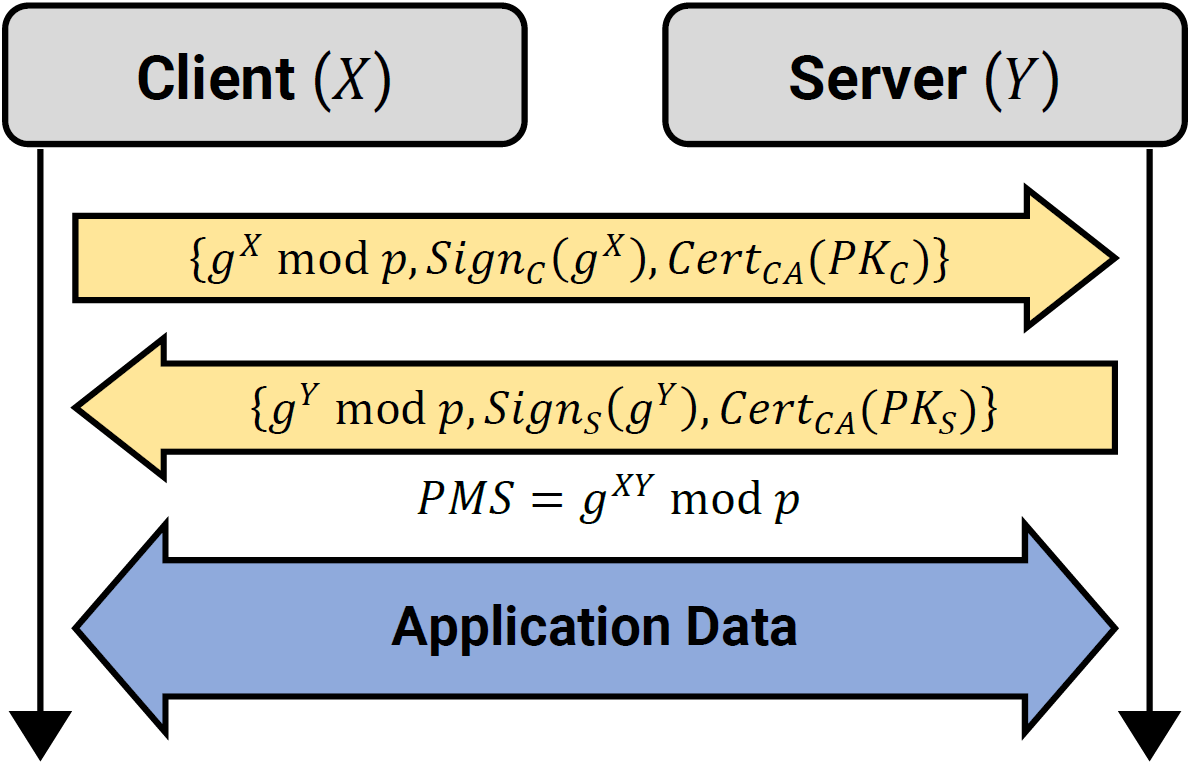
\includegraphics[width=0.7\textwidth]{image/ephdh.png}
    \caption{Ephimeral Diffie Hellman in TLS v.1.3 during Key Exchange}
    \label{fig:ephdh}
\end{figure}
\subsection{Handshake}
L'handshake completo in v1.3 è composto dai seguenti messaggi:
\begin{figure}[h]
    \centering
    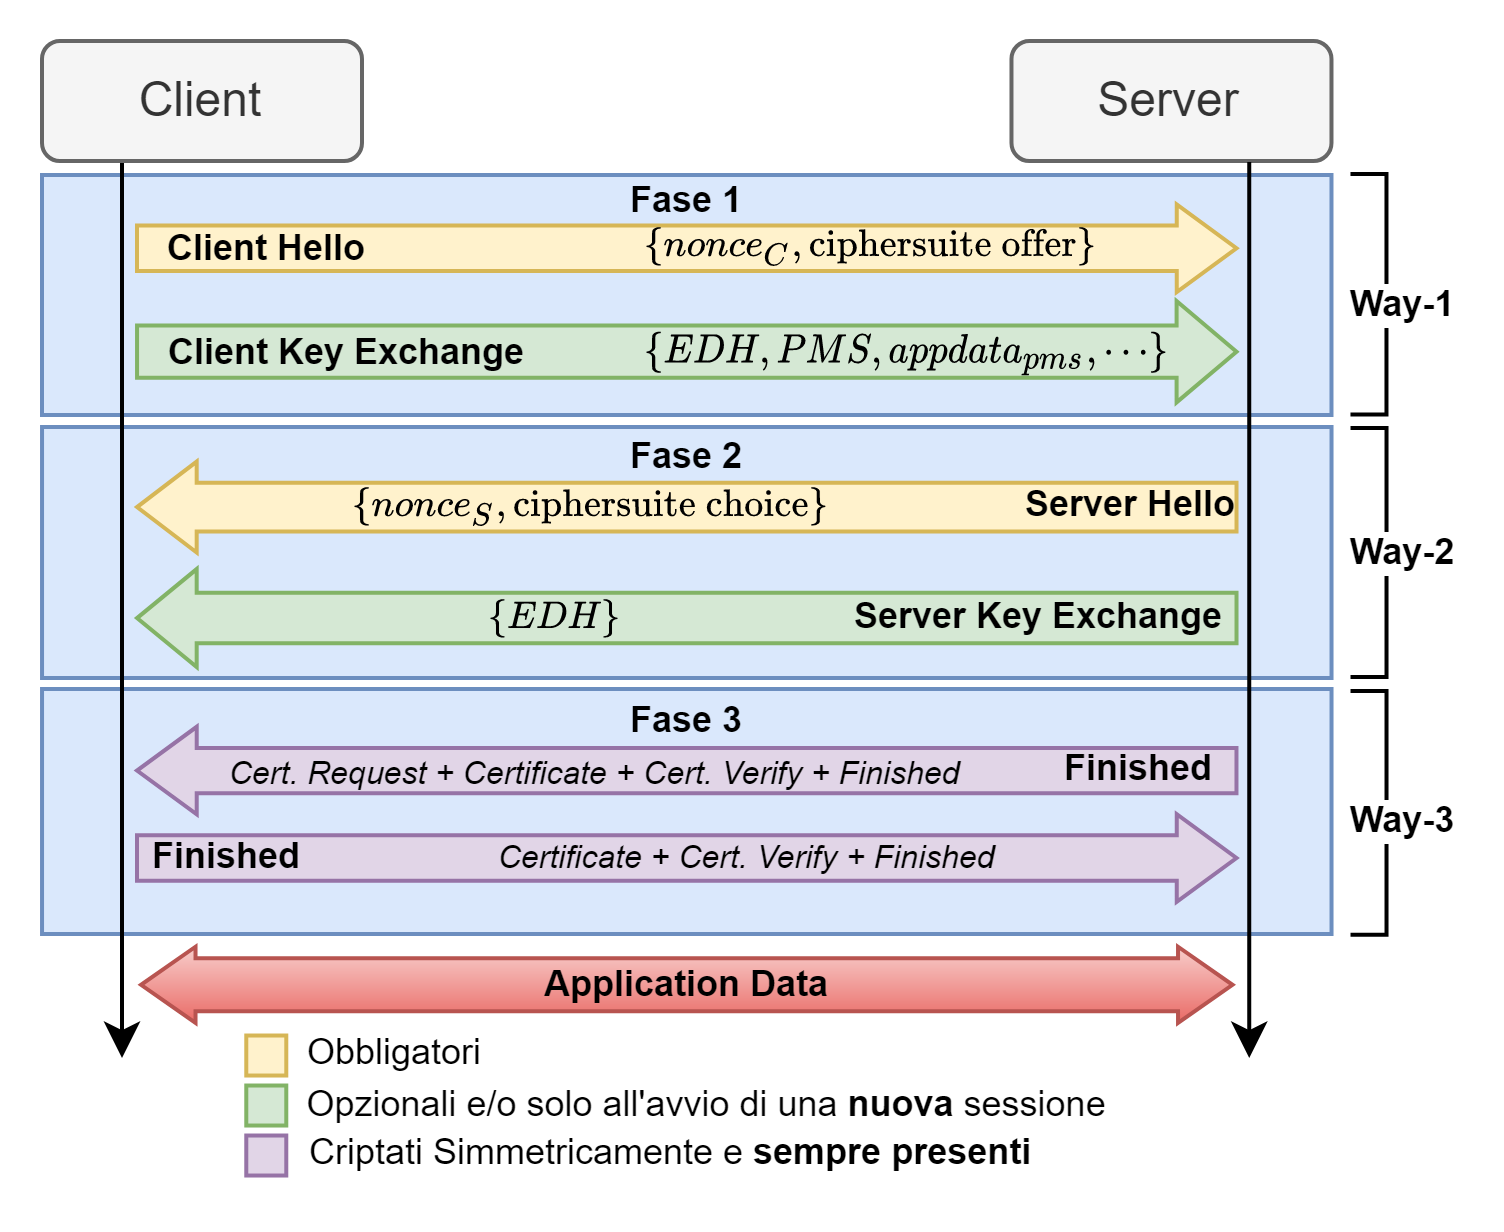
\includegraphics[width=\linewidth]{image/handshakev13.png}
    \caption{TLS v1.3 Handshake Protocol}
    \label{fig:tlshand13}
\end{figure}
\begin{remark}
Come possiamo vedere, avendo \textbf{obbligato} l'uso di \textbf{EDH} per il key agreement, l'\textbf{handshake} ne risulta più \textbf{snello e veloce} in quanto il \textbf{client} \textbf{non deve più aspettare la chiave pubblica del server}, ottenuta tramite il relativo certificato.\\
Inoltre, ci viene garantita la PMS e possiamo criptare immediatamente i certificati, per garantire \textit{\textbf{identity protection}}
\end{remark}
\subsection{Perfect Forward Secrecy con Pre-Shared Key}
TLS v1.3 permette di garantire PFS anche con uso esclusivo \textbf{pre-shared key}, ovvero, permette di \textbf{derivare chiavi di sessione} in maniera \textbf{sicura} e \textbf{senza usare} certificati e firme digitali.
\begin{theorem}[PMS with Pre-Shared Key]
Sia $PSK$ una \textbf{pre-shared key} nota sia al client che al server. \footnotemark \\
Le \textbf{chiavi di sessione} vengono calcolate usando le \textbf{nonces} e \textbf{Anonumous DH} (\cref{def:dh}):
\[\text{Keys}=\text{HKDF}(PSK,label,\{nonce_C,nonce_S,g^{xy}\mod(P)\})\]
\footnotetext{\textsuperscript{\thefootnote}Può essere installata offline o determinata alla prima connessione TLS tra le due parti.}
\end{theorem}
\begin{remark}
Nel caso in cui venga scoperta la PSK, un attaccante \textbf{non è in grado} di recuperare le chiavi di sessioni passate in quanto i valori segreti $X,Y$ cambiano ad ogni \textbf{rekeying} e \textbf{non è computazionalmente} in grado di \textbf{calcolarli} a partire dalla \textbf{conoscenza} di $g^{xy}\mod(P)$
\end{remark}
\begin{remark}
La PSK ha caratteristiche \textbf{simili} al \textbf{PMS}, ma:
\begin{itemize}
    \item Viene utilizzato differentemente nella generazione delle chiavi.
    \item Non viene rigenerato ad ogni nuova sessione TLS.
\end{itemize}
\end{remark}
\subsection{0-RTT Data}
Una caratteristica di TLSv1.3 è la \textbf{possibilità} di effettuare \textbf{0-RTT Data}:
\begin{definition}[0-RTT Data]\label{def:zerortt}
E' una modalità di trasmissione che permette di \textbf{inviare immediatamente dati applicativi} nel primo messaggio di handhsake, nel caso in cui sia \textbf{già} stata \textbf{stabilita} la \textbf{pre-shared key} PSK.
\end{definition}
Le \textbf{chiavi di sessioni} utilizzate per criptare i dati con 0-RTT vengono generati nel seguente modo:
\begin{definition}[0-RTT KeyGen]\label{def:zerorttkey}
\begin{enumerate}
    \item \textbf{Durante} la \textbf{way-1} dell'handshake le chiavi di sessione utilizzate sono calcolate come:
    \[\text{Keys}=\text{HKDF}(PSK,label,\{nonce_C,nonce_S,g^{x}\mod(P)\})\]
    \item Dalla \textbf{way-2} dell'handshake in poi le chiavi di sessione utilizzate sono calcolate come:
    \[\text{Keys}=\text{HKDF}(PSK,label,\{nonce_C,nonce_S,g^{xy}\mod(P)\})\]
\end{enumerate}
\end{definition}
L'inclusione dei coefficienti DH permette di rispettare le condizioni necessarie alla PFS. Tuttavia, le \textbf{chiavi temporanee} di sessione utilizzate nel primo messaggio \textbf{non} inlcudono la \textbf{nonce} ed il coefficiente del server, per cui la way-1 dell'handshake è vulnerabile a replay attack. Alcune possibili mitigazioni sono:
\begin{itemize}
    \item \textbf{Inserire} una \textbf{finestra di validità} per la \textbf{pre-shared key} così da limitare l'intervallo temporale in cui possono avvenire replay attack sull'handshake.
    \item \textbf{Controllare} il \textbf{riuso di nonce} da parte del client, così da individuare replay attacks. Tuttavia, tale soluzione è poco scalabile.
\end{itemize}
